% Project documentation: Retention and Revenue Leakage Analysis (UCI Online Retail II)
% Compile with: pdflatex project_documentation.tex (run twice). Figures are read from ./figures/ (and ../../reports/figures/).
% Tables and key numbers in generated/ are written by notebooks/10_documentation_tables.ipynb: re-run it, do not edit them by hand.
\documentclass[11pt,a4paper]{report}
\usepackage[utf8]{inputenc}
\usepackage[T1]{fontenc}
\usepackage{lmodern}
\usepackage[margin=2.5cm]{geometry}
\usepackage{graphicx}
\usepackage{float}
\usepackage{booktabs}
\usepackage{longtable}
\usepackage{array}
\usepackage{tabularx}
\usepackage[table]{xcolor}
\usepackage{amsmath}
\usepackage{enumitem}
\usepackage{listings}
\usepackage{caption}
\usepackage{fancyhdr}
\usepackage{tikz}
\usetikzlibrary{arrows.meta,positioning}
\usepackage[colorlinks=true,linkcolor=blue!50!black,urlcolor=blue!50!black]{hyperref}

\graphicspath{{figures/}{../../reports/figures/}}
% generated by notebooks/10_documentation_tables.ipynb - do not edit
\newcommand{\kpiGross}{20,476,260}
\newcommand{\kpiTracked}{5,878}
\newcommand{\kpiRepeat}{72}
\newcommand{\kpiYoy}{1.9}
\newcommand{\kpiNewDrop}{41}
\newcommand{\kpiChampCust}{24}
\newcommand{\kpiChampRev}{70}
\newcommand{\kpiFlagged}{1,365}
\newcommand{\kpiFlaggedRev}{808,607}
\newcommand{\kpiExpectedLoss}{490,012}

% generated by notebooks/10_documentation_tables.ipynb - do not edit
\newcommand{\twbxBytes}{80,915}
\newcommand{\twbBytes}{284,961}
\newcommand{\tabBuild}{2026.3.0 (20263.26.1022.1645)}
\newcommand{\nSheets}{25}
\newcommand{\nTiles}{12}
\newcommand{\nCharts}{13}
\newcommand{\nDashboards}{5}
\newcommand{\nDataFiles}{12}

\definecolor{navy}{HTML}{1F2A44}
\newcommand{\file}[1]{\texttt{\detokenize{#1}}}
\renewcommand{\arraystretch}{1.15}
\lstset{basicstyle=\ttfamily\footnotesize,breaklines=true,frame=single,backgroundcolor=\color{black!4}}
\pagestyle{fancy}
\fancyhf{}
\fancyhead[L]{Retention and Revenue Leakage Analysis}
\fancyhead[R]{\leftmark}
\fancyfoot[C]{\thepage}
\tikzset{phase/.style={draw=navy,fill=navy!8,rounded corners=3pt,text width=1.9cm,minimum height=1.3cm,align=center,font=\small}}

\title{Retention and Revenue Leakage Analysis\\[2pt]\large UCI Online Retail II -- Project Documentation\\[2pt]\normalsize The six phases of a data analysis project}
\author{Data analyst portfolio project}
\date{2 November 2026}

\begin{document}
\maketitle

\begin{abstract}
This document describes an end-to-end analysis of 1.03 million cleaned transactions from a UK online giftware retailer (December 2009 to 9 December 2011). It follows the six phases of a data analysis project: Ask, Prepare, Process, Analyze, Share and Act. The central finding is that sales are flat (+\kpiYoy\% for January to November 2011 against the same months of 2010) while new-customer acquisition fell \kpiNewDrop\% (June to November). Customers do not leave after one order: \kpiRepeat\% reorder, and cohort quality has been stable since mid-2010. A small loyal group carries the revenue (RFM Champions: \kpiChampCust\% of customers, \kpiChampRev\% of net revenue), and silence, not slowing order gaps or cancellations, predicts churn. The results are shared as an HTML dashboard and a Tableau workbook (packaged as a \file{.twbx}), both documented here. The analysis shows an association between the acquisition drop and flat sales; it does not prove the cause, and the data cannot say why acquisition fell.
\end{abstract}

\tableofcontents
\listoffigures
\listoftables

%=====================================================================
\chapter{Introduction}
\section{Project at a glance}
\begin{table}[H]
\centering
\begin{tabularx}{\textwidth}{lX}
\toprule
Dataset & UCI Online Retail II (two Excel sheets, 1,067,371 raw rows; 1,027,016 after cleaning) \\
Period & 1 December 2009 to 9 December 2011 \\
Business & UK online retailer of giftware, largely wholesale customers \\
Core question & Why is revenue growth held back, and where is revenue lost? \\
Tools & Python (pandas, seaborn, scipy, statsmodels), SQL (SQLite), Jupyter notebooks, Tableau Desktop 2026.3 Free Edition, HTML/SVG \\
Deliverables & Notebooks 00--11 and a run-all notebook, six SQL scripts, an HTML dashboard, and a packaged Tableau workbook \\
\bottomrule
\end{tabularx}
\caption{Project summary.}
\end{table}

\section{The six phases}
\begin{figure}[H]
\centering
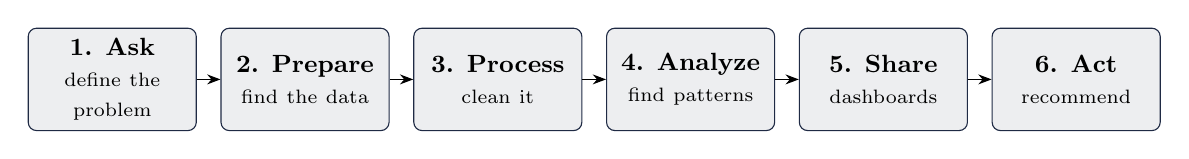
\begin{tikzpicture}[node distance=0.3cm]
\node[phase] (a) {\textbf{1. Ask}\\\scriptsize define the problem};
\node[phase,right=of a] (b) {\textbf{2. Prepare}\\\scriptsize find the data};
\node[phase,right=of b] (c) {\textbf{3. Process}\\\scriptsize clean it};
\node[phase,right=of c] (d) {\textbf{4. Analyze}\\\scriptsize find patterns};
\node[phase,right=of d] (e) {\textbf{5. Share}\\\scriptsize dashboards};
\node[phase,right=of e] (f) {\textbf{6. Act}\\\scriptsize recommend};
\draw[-{Stealth}] (a) -- (b);
\draw[-{Stealth}] (b) -- (c);
\draw[-{Stealth}] (c) -- (d);
\draw[-{Stealth}] (d) -- (e);
\draw[-{Stealth}] (e) -- (f);
\end{tikzpicture}
\caption{The six-phase framework used to structure this document.}
\end{figure}

\begin{table}[H]
\centering
\small
\begin{tabularx}{\textwidth}{llXl}
\toprule
Phase & Chapter & What was produced & Notebooks \\
\midrule
Ask & 2 & 5 Whys, driver tree, success metrics & (docs) \\
Prepare & 3 & Data source, dictionary, quality profile & 00 \\
Process & 4 & Cleaned transactions table with flags & 01 \\
Analyze & 5 & EDA, cohorts, RFM, churn tests, SQL, robustness checks & 02--06, 11 \\
Share & 6 & Sized recommendations, HTML dashboard, Tableau workbook & 07--10 \\
Act & 7 & Action plan, test design, monitoring & -- \\
\bottomrule
\end{tabularx}
\caption{Phases, chapters and project artifacts.}
\end{table}

\section{Repository structure}
\begin{table}[H]
\centering
\small
\begin{tabularx}{\textwidth}{lX}
\toprule
\file{data/raw/} & Downloaded workbook \file{online_retail_II.xlsx} \\
\file{data/processed/} & Cleaned CSV, analysis outputs, \file{retail.db} (SQLite) \\
\file{docs/} & Problem framing (5 Whys, driver tree), data dictionary, this LaTeX source (with generated table fragments) \\
\file{sql/} & Scripts 01--06, run in order \\
\file{notebooks/} & Notebooks 00--11 and \file{run_all.ipynb}, with saved outputs \\
\file{dashboard/} & \file{retail_dashboard.html}, \file{template.html}, \file{tableau/} (workbook and data) \\
\file{reports/figures/} & Charts produced by the notebooks \\
\bottomrule
\end{tabularx}
\caption{Folder layout.}
\end{table}

%=====================================================================
\chapter{Phase 1: Ask}
\section{Business context and question}
The retailer's sales growth is weak. The question is: \emph{why is revenue growth held back, and where is revenue being lost?} The focus is customer retention and repeat purchasing. The only data available is transactions: there is no marketing, channel or web-traffic data.

\section{Hypotheses: the 5 Whys}
The analysis was framed before touching the data. Each ``why'' is a hypothesis to confirm or refute.
\begin{table}[H]
\centering
\small
\begin{tabularx}{\textwidth}{lXXl}
\toprule
\# & Hypothesis & Evidence needed & Verdict \\
\midrule
1 & Too few customers keep buying after their first orders & Cohort retention, repeat rate & Refuted \\
2 & Revenue depends on a small set of customers & Pareto curve, RFM & Confirmed \\
3 & Purchase gaps lengthen before churn & Inter-purchase gap analysis & Refuted \\
4 & Seasonality and cancellations drive churn & Seasonality, cancellation rates, tests & Partly \\
5 & No early-warning signal exists & Back-tested churn rule & Feasible \\
\bottomrule
\end{tabularx}
\caption{5 Whys hypotheses and their final verdicts (details in Chapter~5).}
\end{table}

\section{Driver tree}
\begin{itemize}[nosep]
\item \textbf{Revenue growth stalls or leaks}
  \begin{itemize}[nosep]
  \item Customer base: new customers (acquisition per month); existing customers (retention, churn, concentration)
  \item Order value: basket size, average unit price and product mix
  \item Order frequency: inter-purchase time, seasonality
  \item Leakage: cancellations, returns, guest orders with no customer ID
  \end{itemize}
\end{itemize}

\section{Success metrics}
Repeat purchase rate; monthly cohort retention; revenue share by RFM segment; cancellation rate by value; share of revenue from customers at churn risk.

%=====================================================================
\chapter{Phase 2: Prepare}
\section{Data source}
UCI Online Retail II (\url{https://archive.ics.uci.edu/dataset/502/online+retail+ii}). One Excel workbook with two sheets (\file{Year 2009-2010}: 525,461 rows; \file{Year 2010-2011}: 541,910 rows). Notebook 00 downloads and extracts it into \file{data/raw/}. Customer IDs are anonymised numbers, and no personal data is used.

\section{Data dictionary}
\begin{table}[H]
\centering
\small
\begin{tabularx}{\textwidth}{llX}
\toprule
Column & Type & Description \\
\midrule
Invoice & string & Invoice number; a leading C marks a cancellation \\
StockCode & string & Product code \\
Description & string & Product name \\
Quantity & integer & Units per line (negative for cancellations) \\
InvoiceDate & datetime & Invoice date and time \\
Price & float & Unit price in GBP \\
Customer ID & float & Customer number (missing for guest orders) \\
Country & string & Customer's country \\
\bottomrule
\end{tabularx}
\caption{Raw columns.}
\end{table}

\section{Data quality profile}
\begin{table}[H]
\centering
\begin{tabular}{lr}
\toprule
Issue (raw data) & Rows \\
\midrule
Missing customer ID & 243,007 \\
Missing description & 4,382 \\
Cancellation invoices (start with C) & 19,494 \\
Price $\le 0$ & 6,207 \\
Quantity $\le 0$ & 22,950 \\
Non-product stock codes (postage, fees, vouchers) & 6,093 \\
Exact duplicate rows & 34,335 \\
\bottomrule
\end{tabular}
\caption{Issues found by profiling notebook 01.}
\end{table}

\section{Environment}
Windows 11, Python 3.15.2 in a project virtual environment (pandas, numpy, openpyxl, matplotlib, seaborn, scipy, statsmodels, ipykernel, nbclient, nbconvert). JupyterLab does not install on Python 3.15 because a dependency (\file{pyyaml}) has no build for it; notebooks are run through VS Code or \file{nbconvert}. \file{requirements.txt} pins the tested package versions, \file{requirements-jupyterlab.txt} adds JupyterLab for Python 3.12 or 3.13, and \file{notebooks/run_all.ipynb} runs notebooks 01--09 in order.

%=====================================================================
\chapter{Phase 3: Process}
\section{Cleaning pipeline}
\begin{table}[H]
\centering
\begin{tabular}{lrr}
\toprule
Step & Rows removed & Rows after \\
\midrule
Raw (both sheets) & -- & 1,067,371 \\
Drop December 2010 sheet overlap (verified identical) & 22,523 & 1,044,848 \\
Drop exact duplicates & 11,812 & 1,033,036 \\
Drop price $\le 0$ (samples, adjustments, write-offs) & 6,019 & 1,027,017 \\
Negative quantity on non-cancellations & 0 & 1,027,017 \\
Cancellation with positive quantity (inconsistent) & 1 & 1,027,016 \\
\bottomrule
\end{tabular}
\caption{Row waterfall of notebook 01.}
\end{table}

\section{Design decisions}
\begin{itemize}[nosep]
\item \textbf{Flag, do not drop:} non-product codes (0.57\% of rows) and guest orders (15.1\% of sales value) are flagged so totals stay reconcilable.
\item \textbf{Cancellations are kept} and flagged; net values subtract them.
\item \textbf{Duplicates:} exact duplicates are dropped; some may be genuine repeat scans, which is a documented limitation.
\item \textbf{Derived fields:} line total, cancellation flag, invoice month, and each customer's first-purchase month (the cohort).
\end{itemize}

\section{Result}
The cleaned table has 1,027,016 rows, 48,368 invoices and gross sales of \pounds 20,476,260. Cancelled value is \pounds 1,462,424 (7.1\% of gross sales). Assertions confirm that prices are positive and that cancellations have negative quantities.
\begin{figure}[H]
\centering
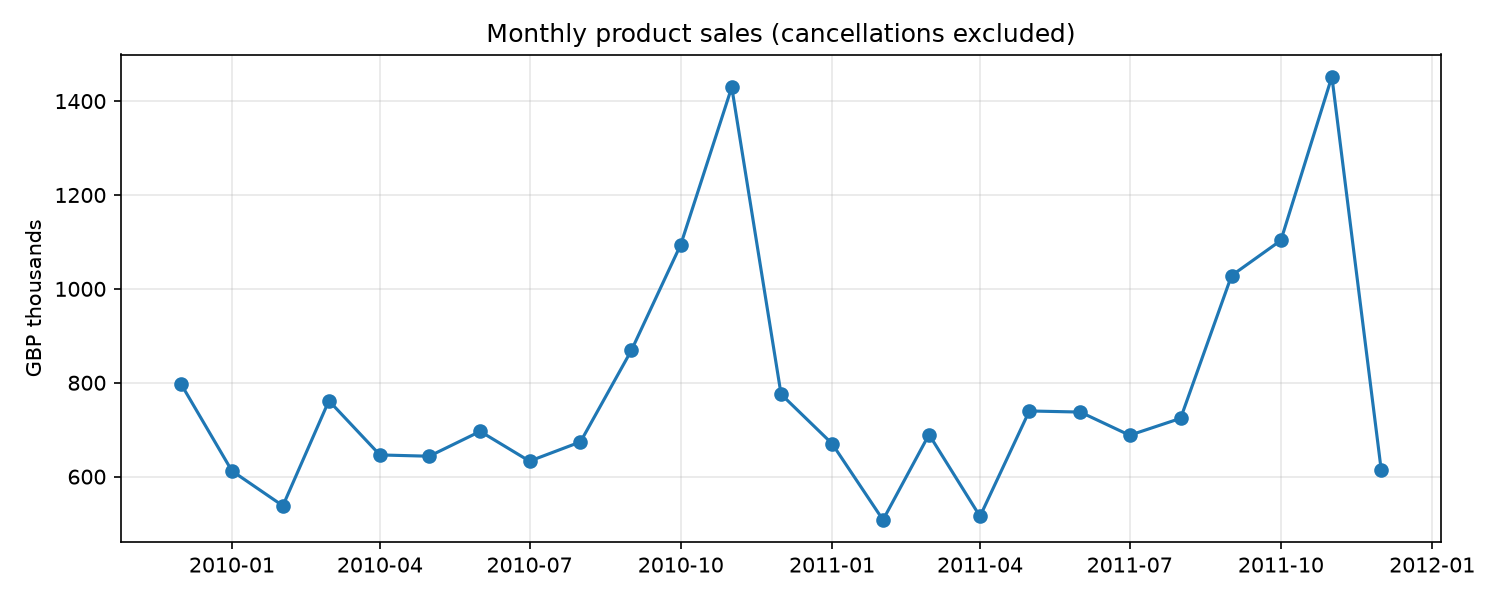
\includegraphics[width=0.85\textwidth]{01_monthly_sales_sanity_check.png}
\caption{Sanity check: monthly product sales after cleaning.}
\end{figure}

%=====================================================================
\chapter{Phase 4: Analyze}
\section{Exploratory analysis (notebook 02)}
\begin{itemize}[nosep]
\item \textbf{Flat sales.} January--November 2011 sales were \pounds 9.18M against \pounds 9.01M in 2010 (+1.9\%). September--November is about 40\% of January--November sales in both years.
\item \textbf{Growth came from existing customers.} Returning-customer sales rose from \pounds 6.24M to \pounds 7.08M, while new-customer sales fell from \pounds 1.56M to \pounds 0.72M.
\item \textbf{Strong repeat behaviour.} 72.4\% of 5,878 tracked customers placed two or more orders; the median gap between orders is 32 days.
\item \textbf{Concentration.} The top 1\%, 5\%, 10\% and 20\% of customers bring 31.8\%, 51.9\%, 63.9\% and 77.2\% of tracked sales.
\item \textbf{Leakage.} Cancellations are 7.1\% of gross sales; 26\% of cancelled value was reversed within an hour (likely entry corrections), and excluding it the rate is 5.4\%. Guest orders are 15\% of sales. The UK is 85\% of sales.
\end{itemize}
\begin{figure}[H]
\centering
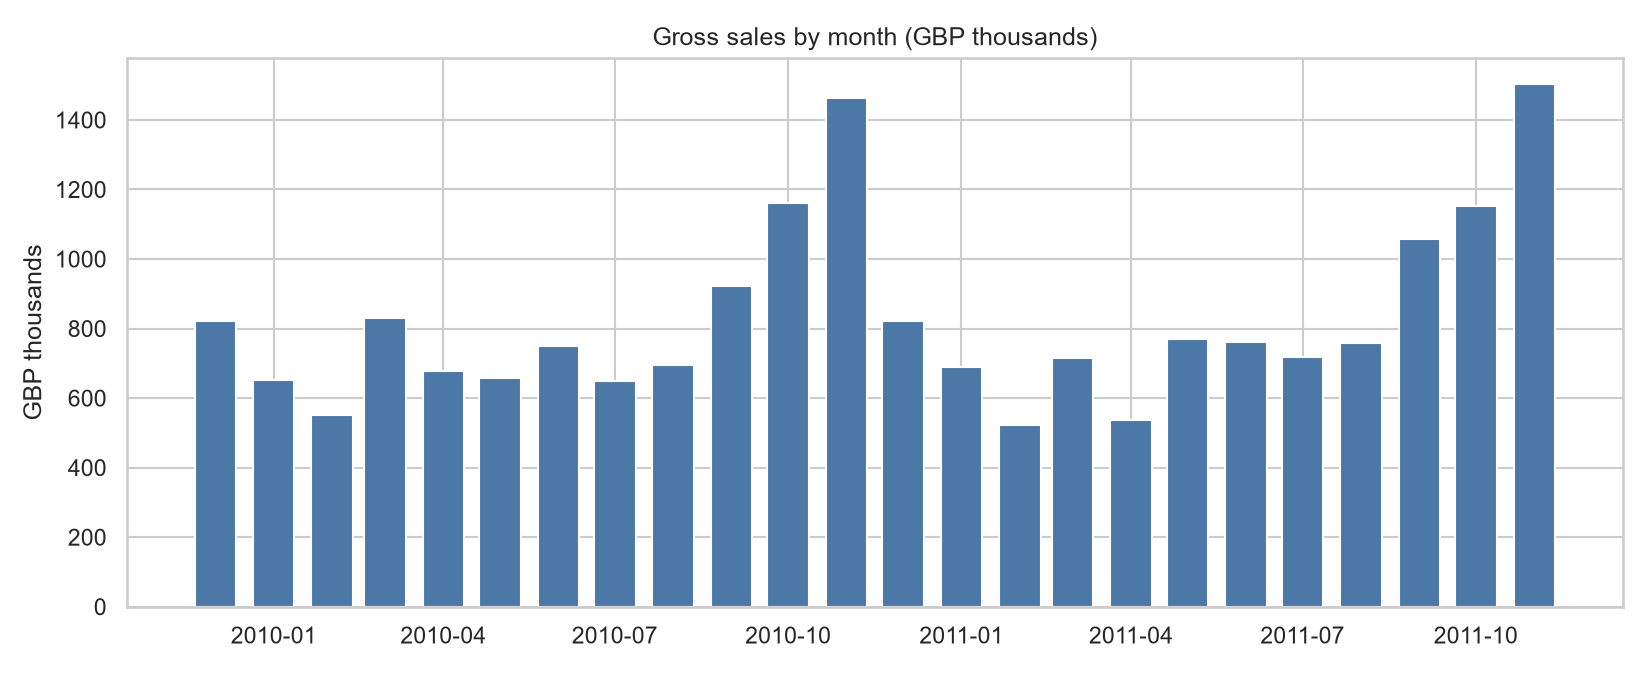
\includegraphics[width=0.85\textwidth]{02_monthly_gross_sales.png}
\caption{Gross sales by month.}
\end{figure}
\begin{figure}[H]
\centering
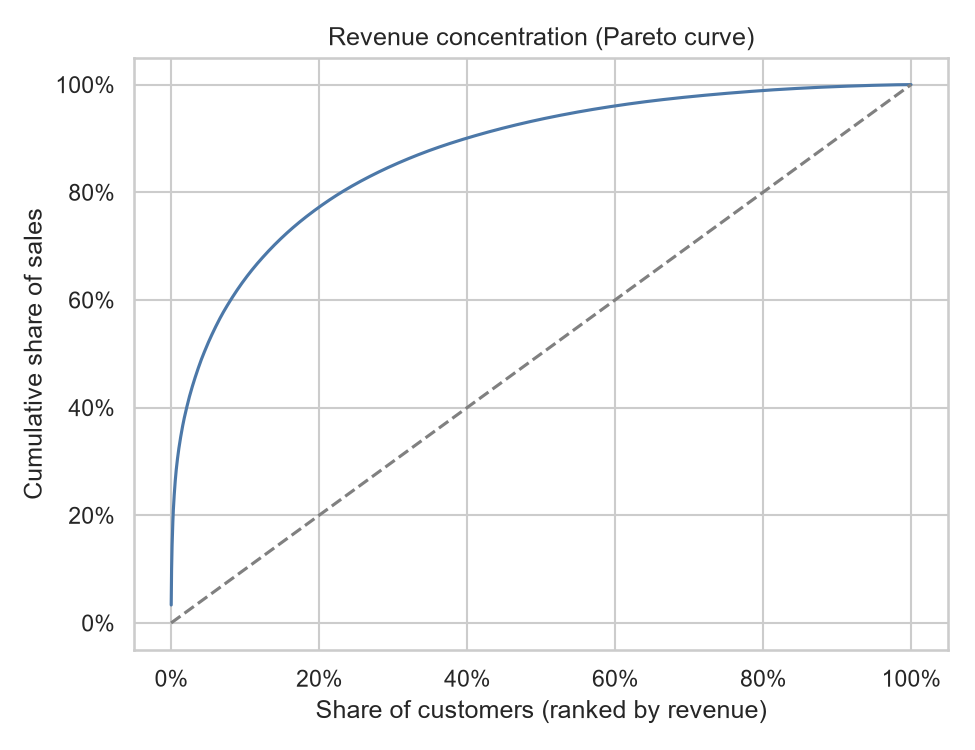
\includegraphics[width=0.85\textwidth]{02_customer_concentration.png}
\caption{Revenue concentration (Pareto curve).}
\end{figure}
\begin{figure}[H]
\centering
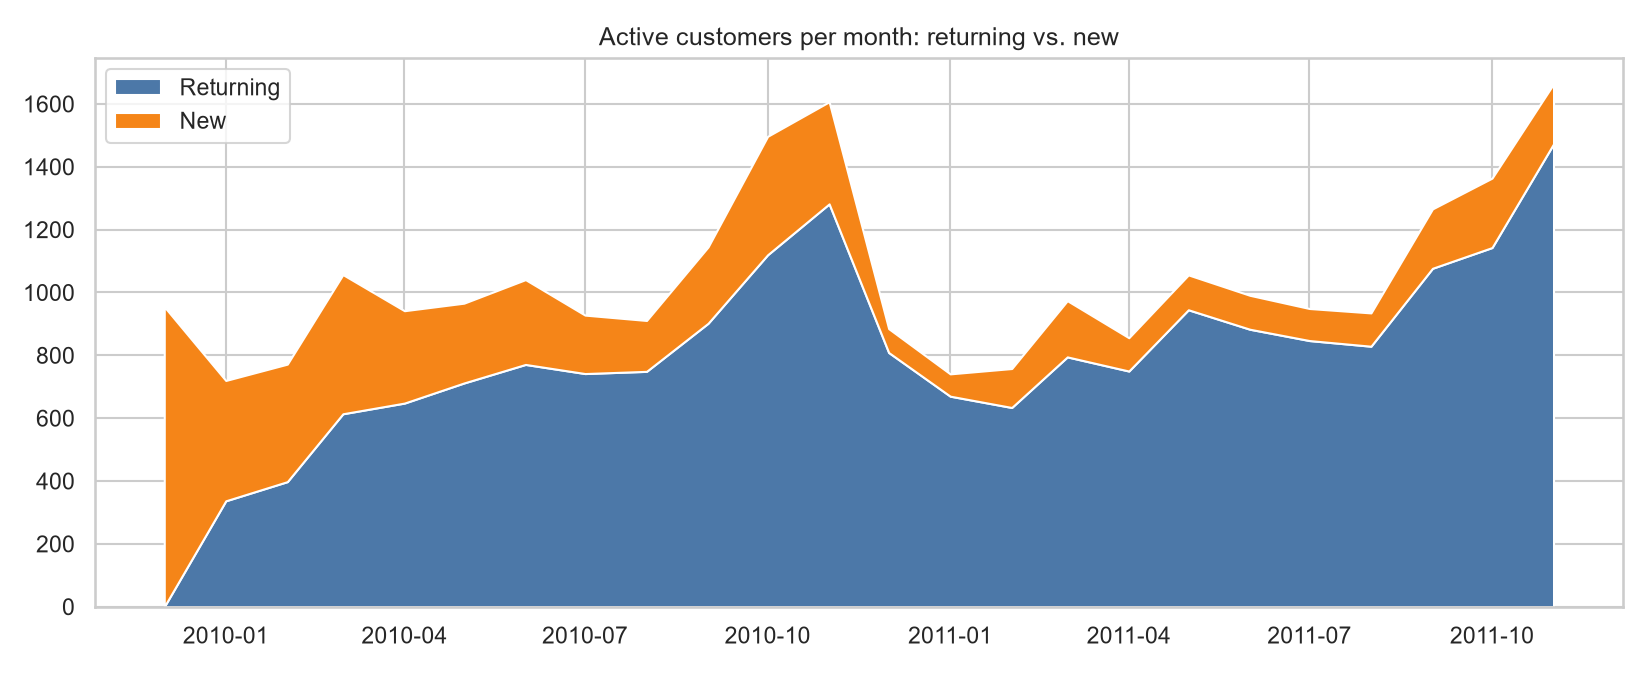
\includegraphics[width=0.8\textwidth]{02_new_vs_returning_customers.png}
\caption{Active customers per month: returning against new.}
\end{figure}
\begin{figure}[H]
\centering
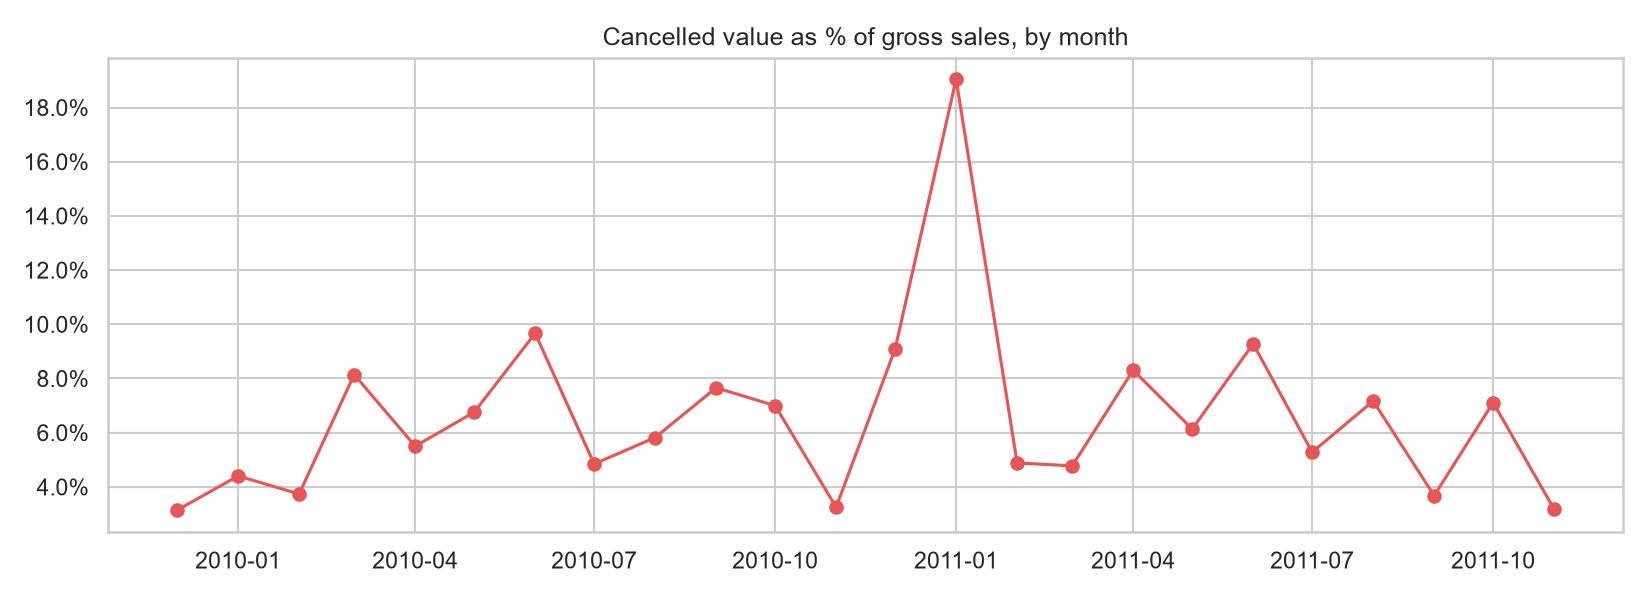
\includegraphics[width=0.8\textwidth]{02_cancellation_rate.png}
\caption{Cancelled value as a share of gross sales, by month.}
\end{figure}
\begin{figure}[H]
\centering
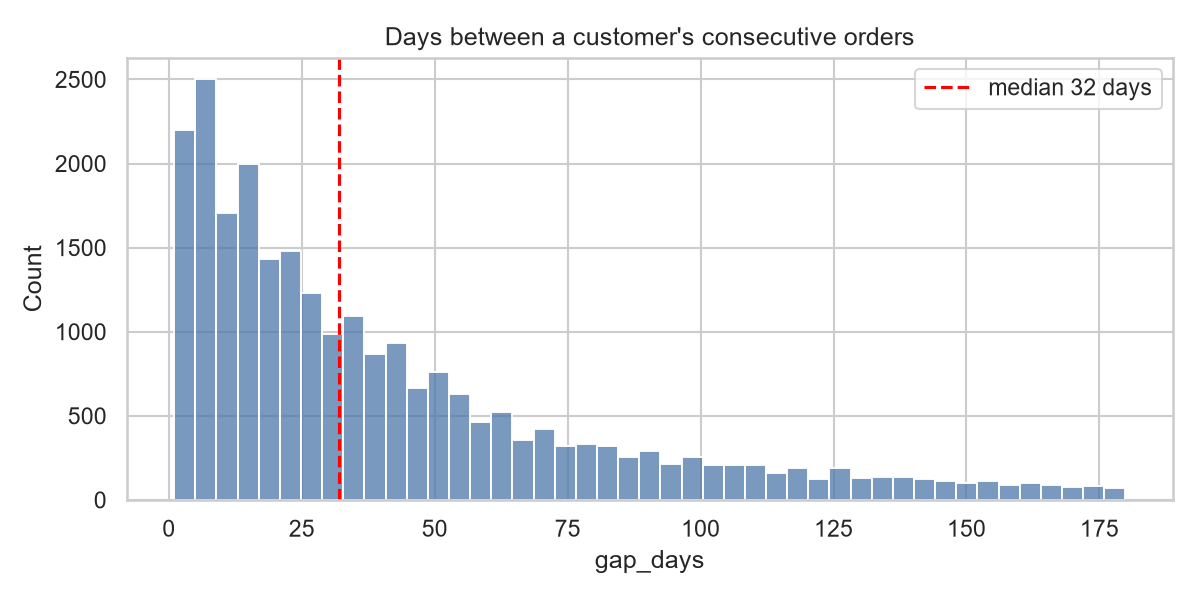
\includegraphics[width=0.8\textwidth]{02_inter_purchase_gap.png}
\caption{Days between a customer's consecutive orders (median 32 days).}
\end{figure}

\section{Cohort retention (notebook 03)}
A customer's cohort is the month of their first purchase; retention in month $k$ means at least one order $k$ months later. Month-1 activity is about 20\% for the 2010 and 2011 cohorts. The 90-day repeat rate is 45\%, 41\% and 41\% for 2010 H1, 2010 H2 and 2011 H1: it dropped about four points ($p=0.013$) between the two halves of 2010 and then held (Section~\ref{sec:robust}). Monthly retention is seasonal: cohorts light up again when the autumn peak returns. New customers for June to November fell from 1,563 (2010) to 917 (2011), a 41\% drop (UK $-43\%$, non-UK $-25\%$); the median first-order value was stable (\pounds 281 to \pounds 300). The December 2009 cohort is overstated because the data starts there.
\begin{figure}[H]
\centering
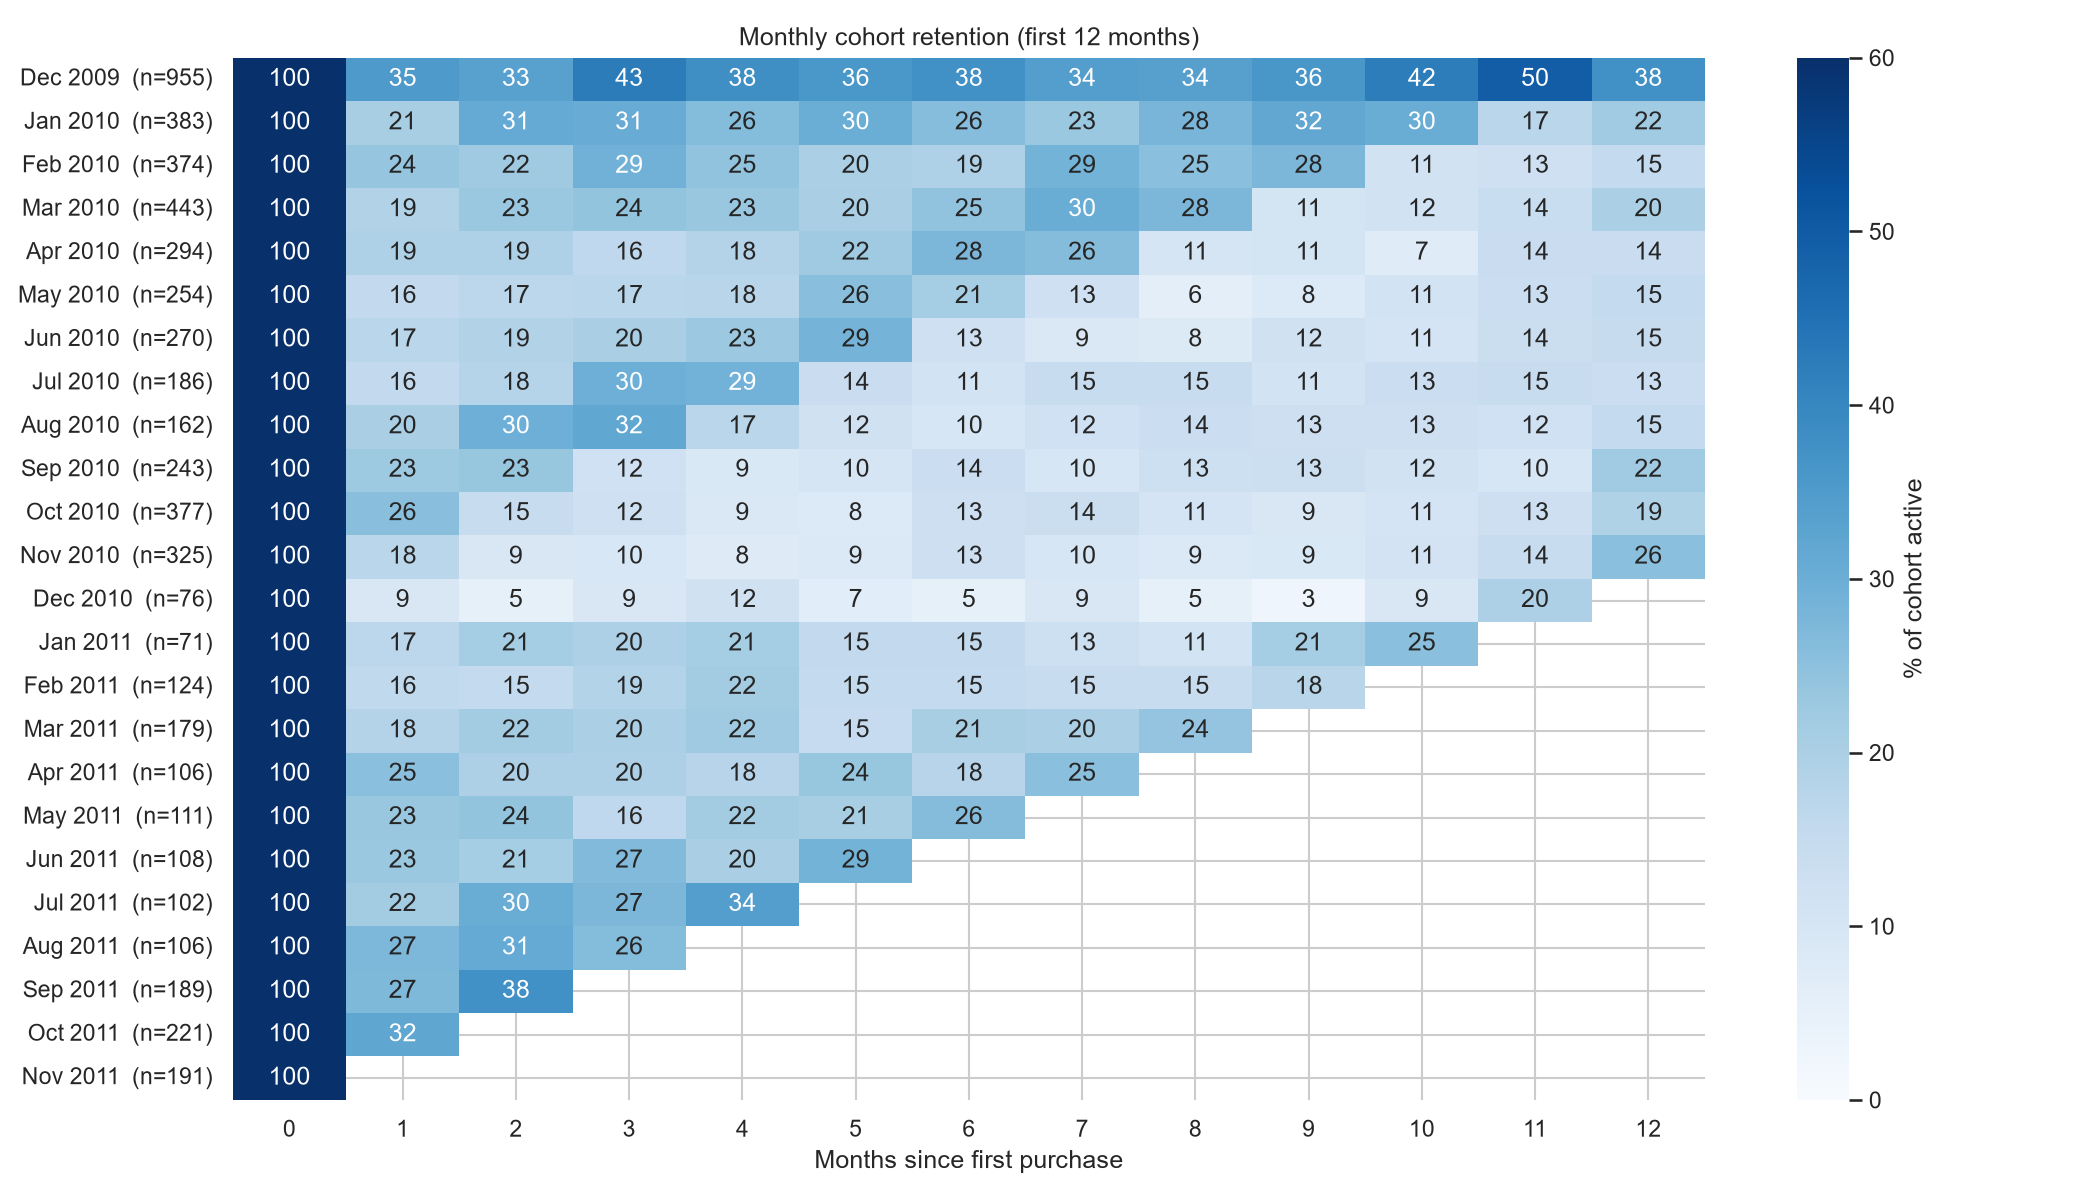
\includegraphics[width=0.95\textwidth]{03_cohort_heatmap.png}
\caption{Monthly cohort retention (first 12 months).}
\end{figure}
\begin{figure}[H]
\centering
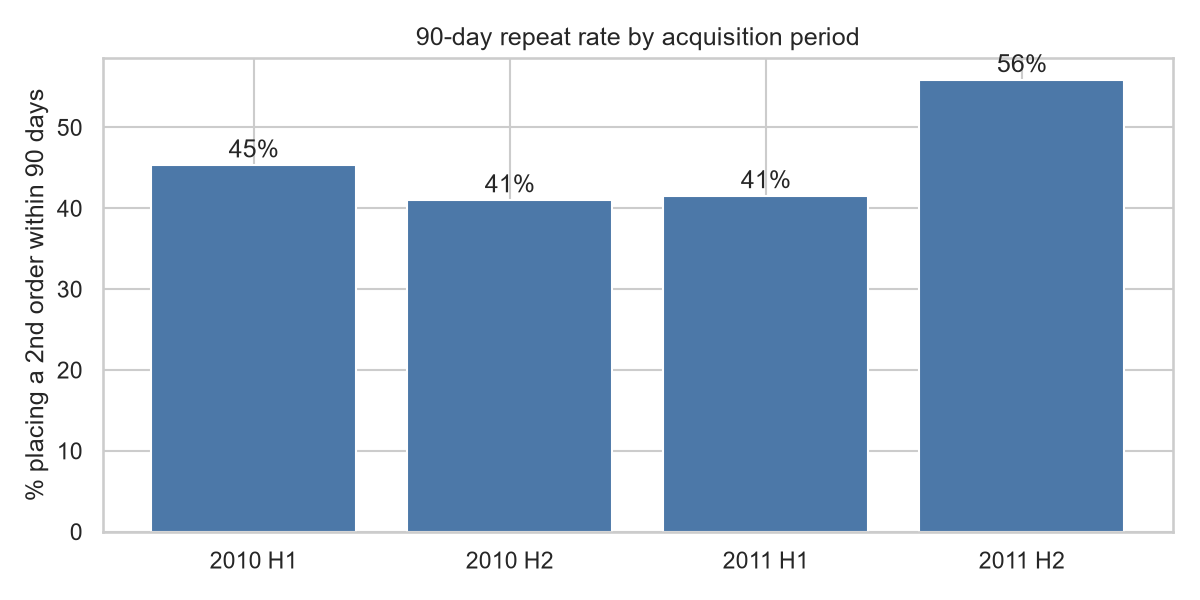
\includegraphics[width=0.8\textwidth]{03_repeat_rate_90d.png}
\caption{90-day repeat rate by acquisition period.}
\end{figure}
\begin{figure}[H]
\centering
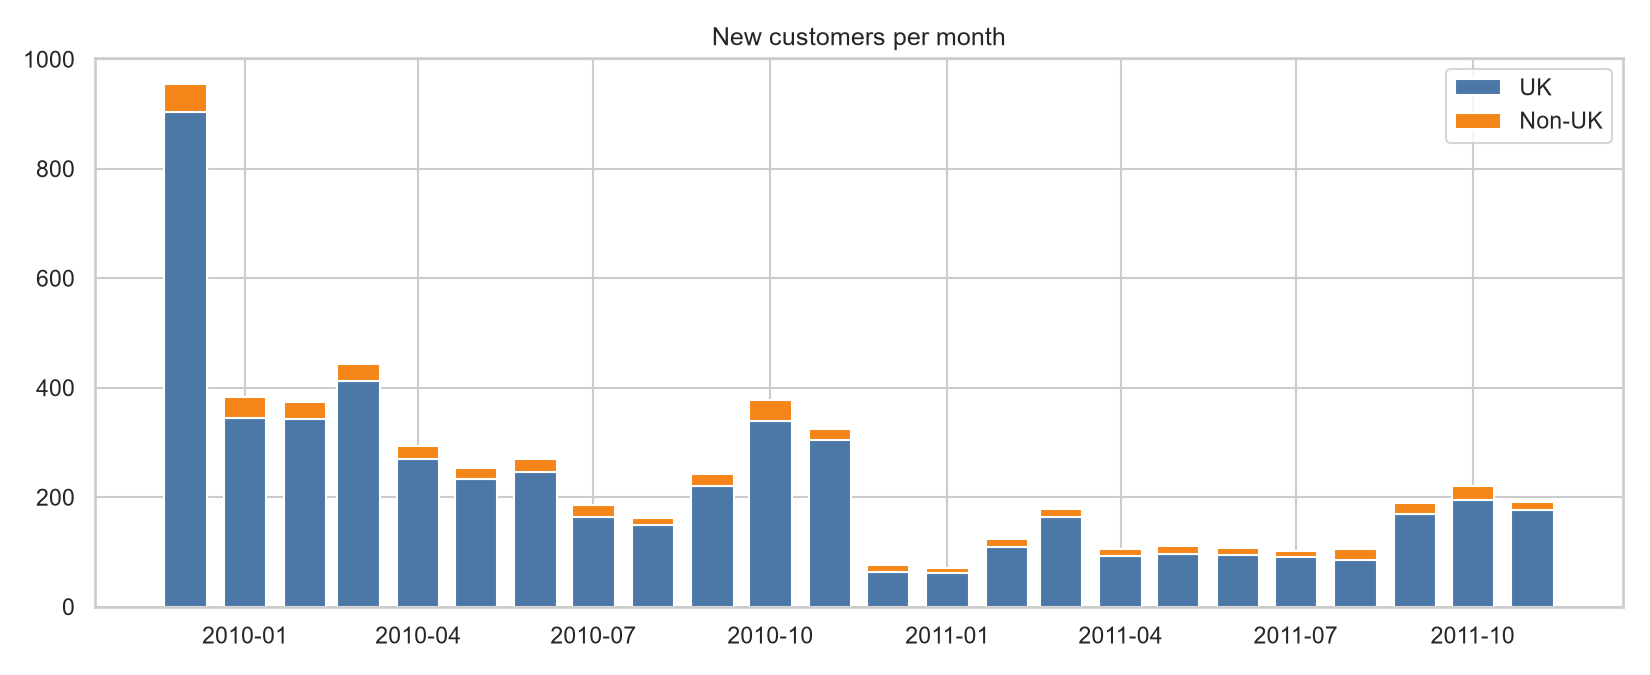
\includegraphics[width=0.8\textwidth]{03_new_customers_per_month.png}
\caption{New customers per month, UK and non-UK.}
\end{figure}

\section{RFM segmentation (notebook 04)}
Recency (days since last order, snapshot 10 December 2011), frequency (distinct invoices) and monetary value (net sales) are scored 1--5. Recency and monetary use quintiles; frequency uses fixed bands (1, 2, 3--4, 5--9, 10+) because quintiles split identical one-order customers arbitrarily. 5,837 customers are scored (41 with net value $\le 0$ are excluded).
\begin{table}[H]
\centering
\small
\begin{tabular}{lrrrr}
\toprule
Segment & Customers & \% customers & Net revenue (\pounds) & \% revenue \\
\midrule
Champions & 1,398 & 24.0 & 11,445,272 & 69.9 \\
Loyal & 472 & 8.1 & 1,632,763 & 10.0 \\
At Risk & 493 & 8.4 & 968,671 & 5.9 \\
Potential Loyalists & 705 & 12.1 & 672,765 & 4.1 \\
Need Attention & 695 & 11.9 & 549,616 & 3.4 \\
Lost & 949 & 16.3 & 384,867 & 2.3 \\
About to Sleep & 674 & 11.5 & 291,886 & 1.8 \\
Can't Lose Them & 67 & 1.1 & 192,344 & 1.2 \\
Hibernating & 152 & 2.6 & 165,904 & 1.0 \\
New Customers & 232 & 4.0 & 78,540 & 0.5 \\
\bottomrule
\end{tabular}

\caption{RFM segments (lifetime net sales within the two-year window, not a forecast).}
\end{table}
Four slipping segments (Need Attention, About to Sleep, At Risk, Can't Lose Them) hold 1,929 customers (33\%) and \pounds 2.0M (12\%) of revenue to date; 126 top-value customers have been silent for 142 days or more (\pounds 858K lifetime sales).
\begin{figure}[H]
\centering
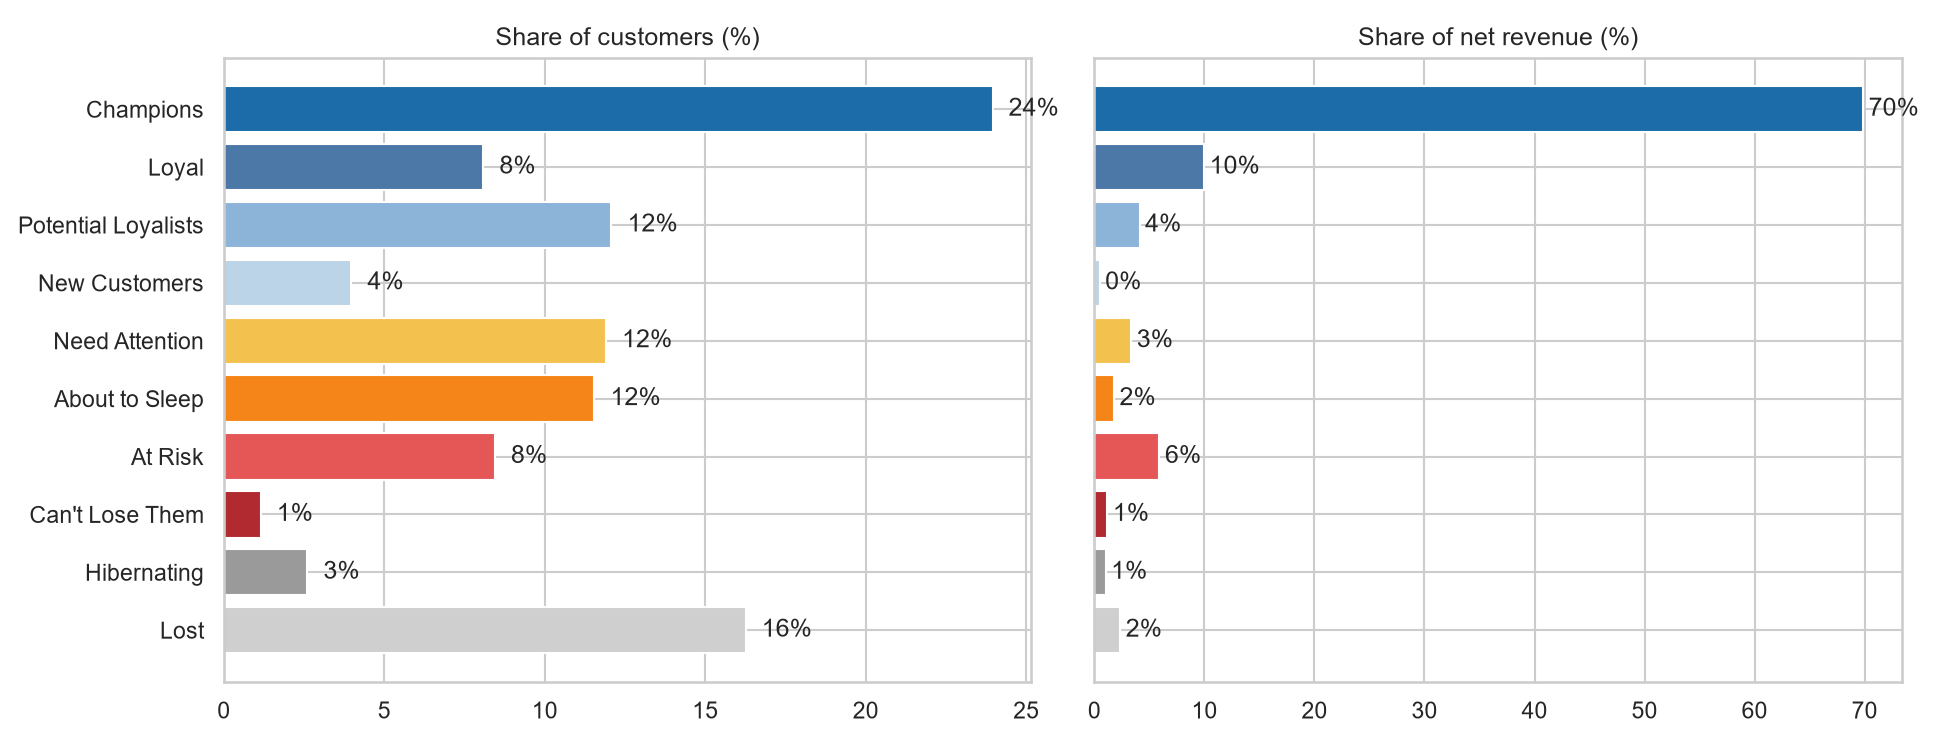
\includegraphics[width=0.8\textwidth]{04_rfm_segments.png}
\caption{RFM segments: share of customers and share of net revenue.}
\end{figure}

\section{Churn and hypothesis tests (notebook 05)}
\textbf{Design.} A time-split back-test: history up to 30 June 2011; base = customers with a purchase in the preceding 12 months (4,326); churned = no purchase in the next 161 days (43.9\% of the base). Features use history only.
\begin{table}[H]
\centering
\begin{tabular}{lrr}
\toprule
Days silent at cutoff & Customers & Churn rate \\
\midrule
0--30 & 1,016 & 18.6\% \\
31--60 & 621 & 25.3\% \\
61--90 & 354 & 38.7\% \\
91--120 & 341 & 46.9\% \\
121--180 & 392 & 53.6\% \\
181--365 & 1,602 & 65.2\% \\
\bottomrule
\end{tabular}

\caption{Churn rises with silence.}
\end{table}
\textbf{Tests} (Mann--Whitney U and chi-square, two-sided).
\begin{itemize}[nosep]
\item Do gaps lengthen before churn? The last gap against earlier gaps does not differ between churners and retained customers ($p=0.58$): \emph{refuted}.
\item Do cancellations drive churn? Customers with cancellations churn less (31.5\% against 54.2\%) because they order more often; after controlling for frequency, value and recency the cancellation rate is not significant ($p=0.54$): \emph{refuted}.
\item A logistic regression (odds ratio per doubling) finds days silent $\times 1.34$, invoices $\times 0.60$ and trailing sales $\times 0.75$; AUC $=0.786$, pseudo-$R^2=0.201$.
\end{itemize}
\textbf{Early-warning rule.} Precision is the share of flagged customers who churned, recall the share of churners flagged, lift the precision divided by the base churn rate.
\begin{table}[H]
\centering
\small
\begin{tabular}{lrrrr}
\toprule
Rule & Flagged & Precision & Recall & Churner revenue caught \\
\midrule
silent $>$ 60 days & 2,689 & 57.7\% & 81.8\% & 74.1\% \\
silent $>$ 90 days & 2,335 & 60.6\% & 74.6\% & 65.1\% \\
silent $>$ 120 days & 1,994 & 62.9\% & 66.1\% & 53.6\% \\
silent $>$ 1.5x own avg gap (3+ orders) & 845 & 43.3\% & 53.4\% & 51.8\% \\
\bottomrule
\end{tabular}

\caption{Selected back-tested rules (full table in \file{data/processed/churn_rule_backtest.csv}).}
\end{table}
Applied at 10 December 2011, the 90-day rule flags 1,365 of 4,264 active customers, worth \pounds 808,607 in trailing 12-month sales; at the back-test precision the expected loss is about \pounds 490,000. Sixty top-tier customers account for \pounds 218,262. Recall at other cutoff dates differs (Section~\ref{sec:robust}), so the 75\% figure applies to the 30 June 2011 cutoff, not in general.
\begin{figure}[H]
\centering
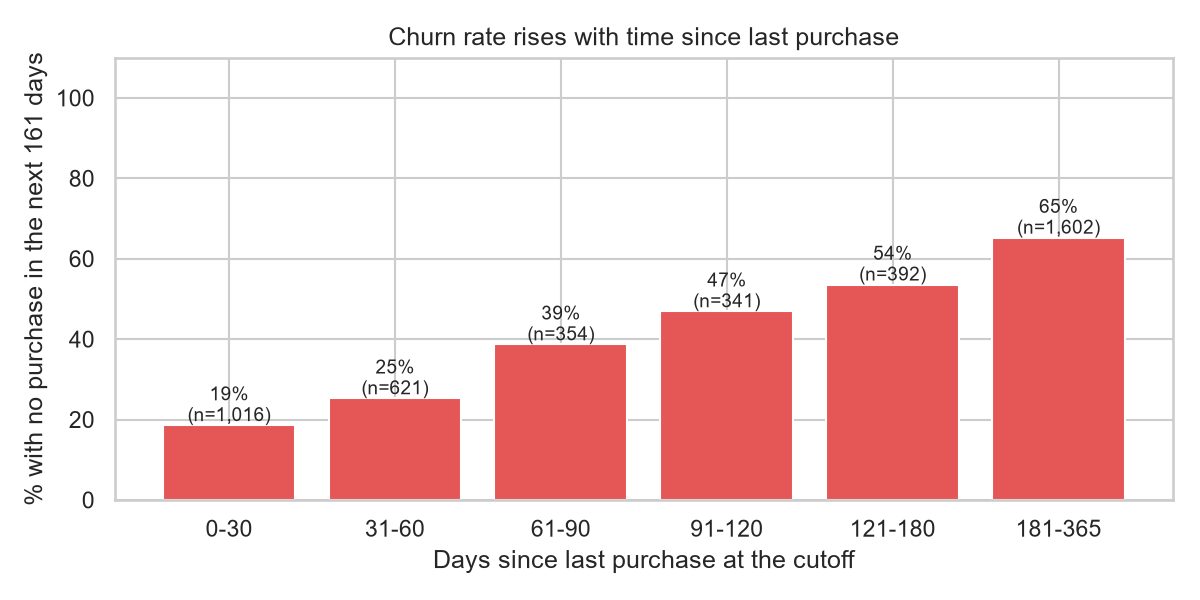
\includegraphics[width=0.75\textwidth]{05_churn_by_recency.png}
\caption{Churn rate by days since last purchase.}
\end{figure}
\begin{figure}[H]
\centering
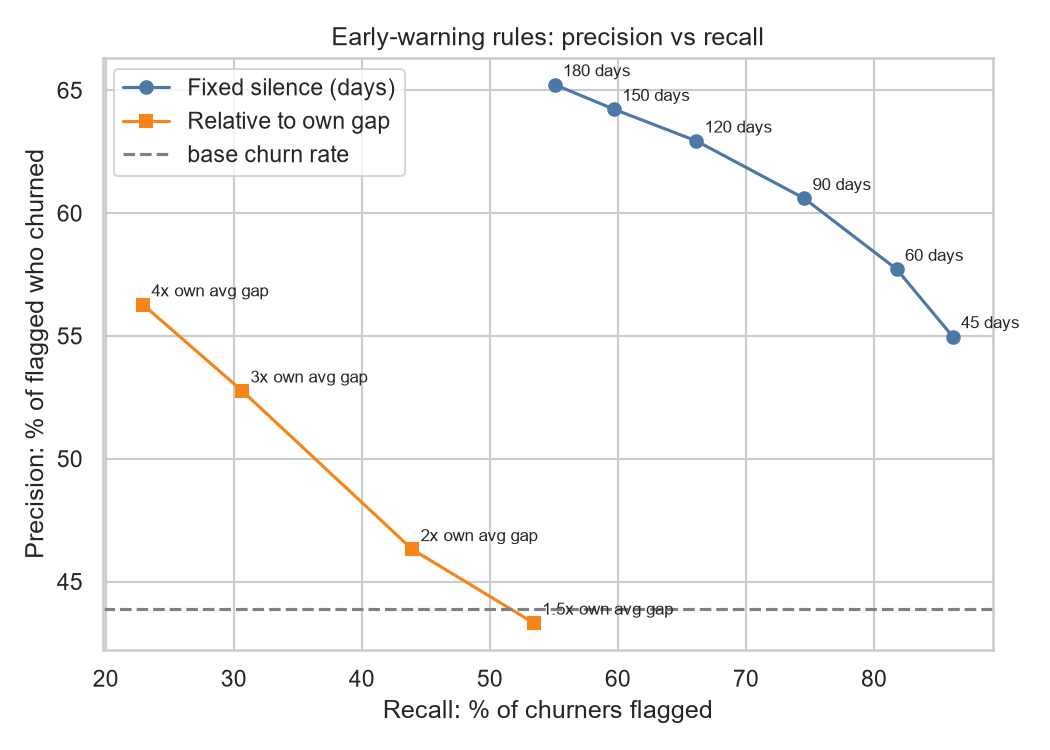
\includegraphics[width=0.7\textwidth]{05_rule_precision_recall.png}
\caption{Early-warning rules: precision against recall.}
\end{figure}

\section{SQL reproduction (notebook 06)}
Six scripts in \file{sql/} (schema, views, KPIs, cohorts, RFM, churn) run on SQLite and use CTEs, window functions (\texttt{LAG}, \texttt{NTILE}, \texttt{ROW\_NUMBER}) and correlated \texttt{EXISTS}. Eighteen reconciliation checks against the pandas results all pass, including all 300 cohort cells.

\section{Robustness checks (notebook 11)}\label{sec:robust}
Three further analyses test how far the main findings can be trusted. They use the same churn label as notebook 05 (no purchase in the 161 days after the cutoff), and the 30 June 2011 results reproduce notebook 05 exactly (4,326 customers, 43.9\% churn).

\subsection{Product mix and churn}
Product categories do not exist in the data, so five features were derived from descriptions and stock codes: the Christmas share of spend (a keyword heuristic), the number of distinct products, the average unit price, units per invoice, and the share of spend on the single biggest product. All five differ between churned and retained customers (Mann--Whitney $p<0.001$), but they overlap with how often and how much a customer buys. Adding them to the logistic model improves the fit (likelihood-ratio $\chi^2=19.7$, 5 degrees of freedom, $p=0.0014$) but barely changes accuracy, and the out-of-time AUC does not move at all. Higher average unit price (odds $\times 1.31$ per doubling, 95\% interval 1.11--1.55) and larger baskets ($\times 1.16$, 1.01--1.32) go with more churn; the Christmas share and the number of products are not significant. Product mix is therefore a small effect that does not change the churn rule.
\begin{table}[H]
\centering
\begin{tabular}{lrr}
\toprule
Measure & Baseline & With product features \\
\midrule
log-likelihood & $-$2,370.0 & $-$2,360.1 \\
AIC & 4,752 & 4,742 \\
pseudo R2 & 0.199 & 0.203 \\
in-sample AUC & 0.786 & 0.788 \\
out-of-time AUC & 0.778 & 0.778 \\
\bottomrule
\end{tabular}

\caption{Churn model with and without the product features (4,318 customers at the 30 June 2011 cutoff; the out-of-time AUC is from a model trained on the November and December 2010 cutoffs).}
\end{table}

\subsection{Stability across cutoff dates}
The back-test was repeated at five cutoffs, each with a 161-day holdout that ends before the data does. The precision of the ``silent $>$ 90 days'' rule is between 61\% and 76\% and is lowest at the original cutoff, but \emph{recall is not stable}: 45\% and 49\% at the two 2010 cutoffs against 75\%--76\% at the three later ones. Base churn falls from 55\% to 44\% because the later holdouts include the autumn peak, when seasonal buyers return. The own-gap rule (1.5 times a customer's own average gap, 3+ orders) keeps a lift of 1.3 to 1.6 at every cutoff. The rule remains useful, but ``catches 75\% of churners'' describes the 30 June 2011 cutoff, not every date.
\begin{table}[H]
\centering
\scriptsize
\begin{tabular}{lrrrrrr}
\toprule
Cutoff & Base & Churn rate & Precision ($>$ 90 d) & Recall ($>$ 90 d) & Revenue caught & Own-gap lift \\
\midrule
2010-11-30 & 4,266 & 54.6\% & 75.5\% & 44.7\% & 34.9\% & 1.56 \\
2010-12-31 & 4,231 & 54.8\% & 72.0\% & 49.1\% & 39.2\% & 1.33 \\
2011-02-28 & 4,276 & 53.0\% & 67.3\% & 76.0\% & 62.8\% & 1.29 \\
2011-04-30 & 4,332 & 50.6\% & 67.3\% & 74.6\% & 65.3\% & 1.46 \\
2011-06-30 & 4,326 & 43.9\% & 60.6\% & 74.6\% & 65.7\% & 1.55 \\
\bottomrule
\end{tabular}

\caption{The churn back-test at five cutoff dates.}
\end{table}
\begin{figure}[H]
\centering
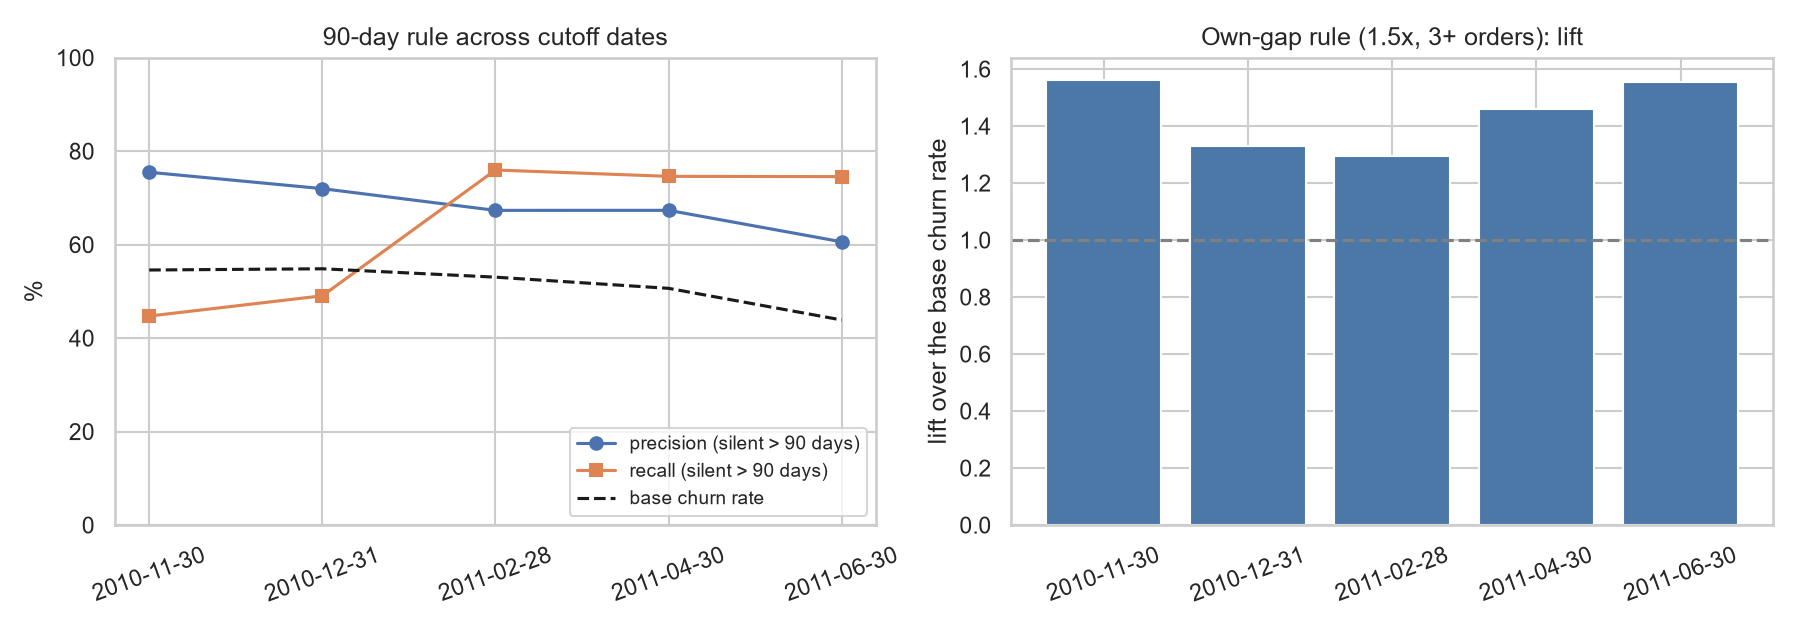
\includegraphics[width=0.9\textwidth]{11_cutoff_stability.png}
\caption{Precision, recall and base churn of the 90-day rule (left) and the lift of the own-gap rule (right) at five cutoffs.}
\end{figure}

\subsection{Uncertainty around the headline numbers}
Customers were resampled with replacement (a cluster bootstrap) because one customer's orders are not independent; sales growth also resamples guest invoices. The repeat rate, the top-10\% share and the rule metrics have narrow intervals. Sales growth of $+1.9\%$ has a 95\% interval from $-4.9\%$ to $+9.7\%$: ``flat'' is supported, but growth cannot be told apart from zero. The 41\% drop in new customers has an exact interval of $-46.0\%$ to $-36.3\%$, and 2011 is below 2010 in all six months (sign test $p=0.031$). The 90-day repeat rate was 45.3\% for 2010 H1 and 41.0\% for 2010 H2 ($p=0.013$), then 41.5\% for 2011 H1 ($p=0.82$ against 2010 H2): cohort quality fell about four points in 2010 and then held. Part of that drop may come from left-censoring, because customers first seen in early 2010 can include people who bought before the data starts. The sampling intervals are much narrower than the cutoff-to-cutoff variation above, so the timing of the back-test matters more than sampling noise.
\begin{table}[H]
\centering
\small
\begin{tabularx}{\textwidth}{Xrrl}
\toprule
Metric & Estimate & 95\% interval & Method \\
\midrule
Repeat purchase rate (2+ orders) & 72.4\% & 71.2\% to 73.5\% & bootstrap \\
Sales growth, Jan-Nov 2011 vs 2010 & +1.9\% & $-$4.9\% to +9.7\% & bootstrap \\
Top 10\% of customers' share of sales & 63.9\% & 59.5\% to 67.8\% & bootstrap \\
Base churn rate (161-day holdout) & 43.9\% & 42.4\% to 45.3\% & bootstrap \\
90-day rule: precision & 60.6\% & 58.6\% to 62.6\% & bootstrap \\
90-day rule: recall & 74.6\% & 72.7\% to 76.3\% & bootstrap \\
New customers Jun-Nov, 2011 vs 2010 & $-$41.3\% & $-$46.0\% to $-$36.3\% & exact binomial \\
90-day repeat rate, acquired 2010 H1 & 45.3\% & 43.1\% to 47.5\% & Wilson \\
90-day repeat rate, acquired 2010 H2 & 41.0\% & 38.4\% to 43.6\% & Wilson \\
90-day repeat rate, acquired 2011 H1 & 41.5\% & 37.9\% to 45.2\% & Wilson \\
\bottomrule
\end{tabularx}

\caption{Headline numbers with 95\% intervals (generated from the notebook 11 results).}
\end{table}
\begin{figure}[H]
\centering
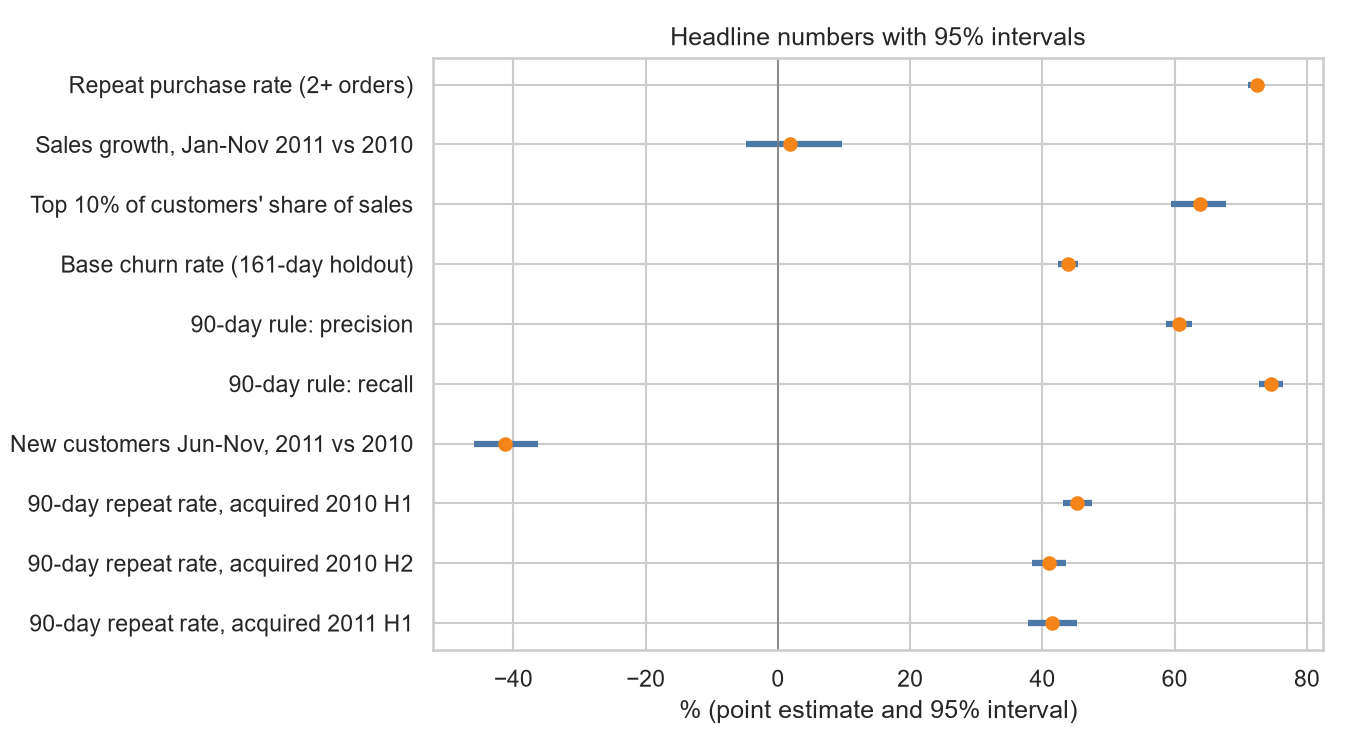
\includegraphics[width=0.8\textwidth]{11_headline_intervals.png}
\caption{Headline numbers with 95\% intervals.}
\end{figure}

\textbf{Caveats.} The cutoffs overlap in time and share customers, so they are not independent tests; bootstrap intervals capture sampling noise only; the new-customer interval assumes arrivals behave like Poisson counts (the sign test needs fewer assumptions); and no adjustment was made for multiple comparisons.

\section{Limits of the analysis}
No marketing data, so the cause of the acquisition drop is unknown. Churn is defined as 161 days without a purchase (a window that includes the autumn peak), not as a confirmed loss. Product mix has only a small association with churn (Section~\ref{sec:robust}); product categories are derived from descriptions and stock codes, not an official field.

%=====================================================================
\chapter{Phase 5: Share}
\section{Recommendations (notebook 07)}
Each recommendation has a measured base taken from the data and a low, mid and high scenario. The scenario percentages are assumptions, not forecasts.
\begin{table}[H]
\centering
\small
\begin{tabularx}{\textwidth}{lXrrrr}
\toprule
\# & Action & Base & Low & Mid & High \\
\midrule
1 & Win back high-value customers silent for more than 90 days & \pounds{}490K & \pounds{}49K & \pounds{}98K & \pounds{}147K \\
2 & Protect Champions and Loyal buyers with a per-customer reorder alert (1.5x their own average gap) & \pounds{}6,677K & \pounds{}67K & \pounds{}134K & \pounds{}200K \\
3 & Find out why new-customer acquisition fell 41\% and restore it (UK first) & \pounds{}371K & \pounds{}93K & \pounds{}186K & \pounds{}371K \\
4 & Add order-entry checks for sale-then-cancel errors and capture customer IDs on guest orders & \pounds{}731K & \pounds{}73K & \pounds{}146K & \pounds{}219K \\
\bottomrule
\end{tabularx}

\caption{Annual impact in GBP (thousands, K) under scenario assumptions; generated from the recommendations output.}
\end{table}
\begin{figure}[H]
\centering
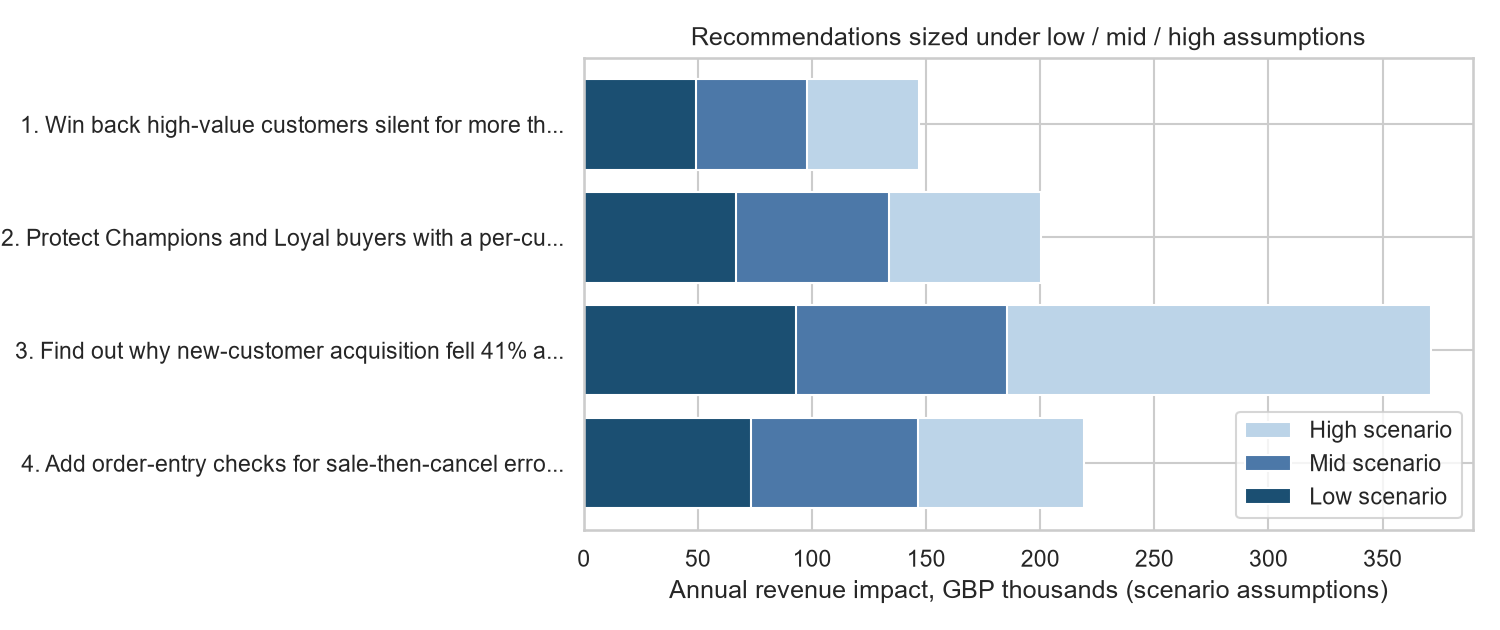
\includegraphics[width=0.8\textwidth]{07_recommendation_impact.png}
\caption{Recommendations sized under low, mid and high scenario assumptions.}
\end{figure}

\section{HTML dashboard}
\file{dashboard/retail_dashboard.html} is a single self-contained file (no server, no internet) with five tabs (Overview, Retention, Segments, Churn risk, Actions), hover tooltips, a table view for every chart and a light/dark theme. It is built by notebook 08 from \file{template.html}.

\section{Tableau packaged workbook}
This section documents \file{dashboard/tableau/retail_dashboard.twbx}, inspected directly from the package.

\subsection{Package structure}
A \file{.twbx} is a zip file. This one (\twbxBytes{} bytes) contains \file{retail_dashboard.twb} (the workbook XML, \twbBytes{} bytes) and \nDataFiles{} CSV files under \file{Data/retail_dashboard/}. The workbook was saved by Tableau \tabBuild{} (Windows, Free Edition licence, workbook schema version 18.1). It starts from the workbook generated by notebook 09 and was later \textbf{re-saved in Tableau with manual edits} (Section~\ref{sec:edits}).

\subsection{Data sources}
Each of the \nDataFiles{} data sources is a text-file connection to a CSV inside the package (relative folder \file{Data/retail_dashboard}), so the package opens on any computer with Tableau.
\begin{table}[H]
\centering
\scriptsize
\begin{tabular}{lrrl}
\toprule
File & Rows & Columns & Data source \\
\midrule
\file{headline_kpis.csv} & 1 & 21 & Headline KPIs \\
\file{monthly_gross_sales.csv} & 24 & 3 & Monthly sales \\
\file{customers_existing_vs_new.csv} & 48 & 3 & Existing vs new customers \\
\file{new_customers_domestic_overseas.csv} & 46 & 3 & New customers by region \\
\file{cohort_heatmap.csv} & 210 & 5 & Cohort retention \\
\file{repeat_rate_90_days.csv} & 5 & 2 & 90-day repeat rate \\
\file{segment_shares_pct.csv} & 20 & 4 & RFM segment shares \\
\file{revenue_concentration_pct.csv} & 101 & 2 & Revenue concentration \\
\file{churn_by_silence.csv} & 6 & 3 & Churn by days silent \\
\file{rule_table.csv} & 10 & 6 & Early-warning rules \\
\file{contact_list.csv} & 12 & 7 & Contact list \\
\file{recommendations_table.csv} & 4 & 7 & Recommendations \\
\bottomrule
\end{tabular}

\caption{Data files inside the package.}
\end{table}

\subsection{Dashboards}
All five dashboards are fixed-size canvases, 1,280 pixels wide, with a navy header banner carrying a one-line takeaway.
\begin{table}[H]
\centering
\small
\begin{tabularx}{\textwidth}{llrX}
\toprule
Dashboard & Size & Sheets & Banner headline \\
\midrule
Actions & 1280$\times$650 & 1 & ``Four moves, sized under low, mid and high scenarios'' \\
Churn risk & 1280$\times$1040 & 7 & ``Silence is the signal: contact customers quiet for 90+ days, biggest first'' \\
Overview & 1280$\times$1040 & 8 & ``Sales are flat while new-customer acquisition fell 41\%'' \\
Retention & 1280$\times$1090 & 3 & ``Cohort quality is stable since mid-2010; acquisition volume is what fell'' \\
Segments & 1280$\times$990 & 5 & ``24\% of customers bring 70\% of revenue'' \\
\bottomrule
\end{tabularx}

\caption{Dashboards in the packaged workbook (read from the file).}
\end{table}
Contents of each dashboard:
\begin{itemize}[nosep]
\item \textbf{Overview:} five headline tiles; year-over-year line charts for gross sales and for new customers (2011 against 2010); existing vs new customers (stacked bars); \emph{Key insights} card.
\item \textbf{Retention:} cohort heatmap; 90-day repeat rate; new customers by region; \emph{What to notice} card.
\item \textbf{Segments:} RFM segment shares; concentration curve; three tiles; \emph{Who is slipping away?} card.
\item \textbf{Churn risk:} four tiles; churn by silence; rule back-test; contact list.
\item \textbf{Actions:} recommendations table; \emph{What this data cannot tell you} card.
\end{itemize}

\subsection{Worksheets}
The workbook has \nSheets{} worksheets: \nTiles{} headline tiles (text marks on the \emph{Headline KPIs} source) and \nCharts{} charts and tables.
\begin{table}[H]
\centering
\small
\begin{tabular}{llp{6.3cm}}
\toprule
Worksheet & Mark & Purpose \\
\midrule
Monthly sales & Bar & Gross sales by month (kept in the workbook; not on the packaged Overview) \\
Monthly sales (2) & Line & Gross sales by calendar month, 2011 against 2010 (added in Tableau) \\
New vs returning & Bar & Existing and new customers per month \\
New vs returning (2) & Line & New customers by calendar month, 2011 against 2010 (added in Tableau) \\
Cohort heatmap & Square & Retention by cohort and month \\
Repeat 90d & Bar & 90-day repeat rate by acquisition period \\
New customers by region & Bar & New customers, domestic and overseas \\
RFM segments & Bar & Customer and revenue shares by segment \\
Concentration & Line & Cumulative share of sales by share of customers \\
Churn by silence & Bar & Churn rate by days silent \\
Rule back-test & Text & Precision, recall and revenue caught per rule \\
Contact list & Text & Top-value customers to contact first \\
Recommendations & Text & Sized recommendations \\
\bottomrule
\end{tabular}

\caption{Chart and table worksheets (the \nTiles{} tile sheets are named ``T \dots'').}
\end{table}

\subsection{Edits made in Tableau}\label{sec:edits}
Compared with the workbook generated by notebook 09, the packaged file contains two worksheets added in Tableau, \emph{Monthly sales (2)} and \emph{New vs returning (2)}. Both are line charts with the calendar month on the axis, one line per year (filtered to 2010 and 2011), colour by year, a year legend in the title and custom tooltips; the second is filtered to new customers. On the Overview, the first replaces the original monthly bar chart. The Overview is 1,040 pixels tall (1,010 in the generated version). Notebook 09 now writes only \file{retail_dashboard_generated.twb} and \file{.twbx}, so re-running it never overwrites this hand-edited file.

\subsection{Design system and technical notes}
Page grey \texttt{\#F3F4F6}; white cards with a thin border; navy banner \texttt{\#1F2A44}; Tableau's default blue and orange for series. Tableau Desktop Free Edition ignores custom colour palettes, so default colours are used. Percentages and millions are pre-scaled in the data because custom axis number formats were unreliable and Tableau applies the viewer's regional separators. Tableau caches an extract per CSV file name; if a CSV's columns change, save it under a new name or the workbook fails with ``InsertData: unbound column''.
\subsection{Dashboard gallery}
The figures show each dashboard as rendered in Tableau Desktop. The window crops the right-most 3\% of the 1,280-pixel canvas, and the bottom of some dashboards may be cut off.
\begin{figure}[H]
\centering
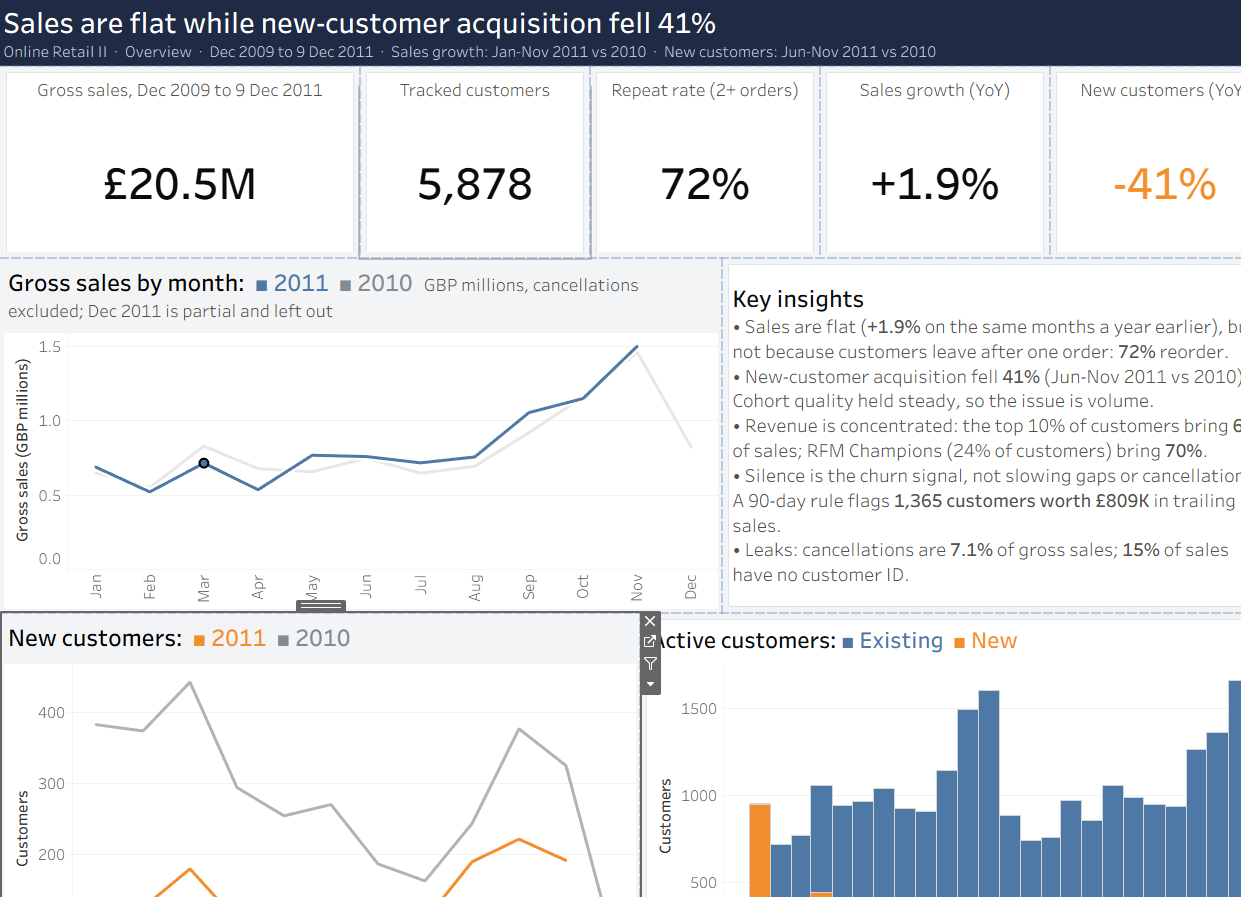
\includegraphics[width=0.95\textwidth]{tableau_overview.png}
\caption{Overview dashboard (packaged workbook, including the year-over-year line charts added in Tableau).}
\end{figure}
\begin{figure}[H]
\centering
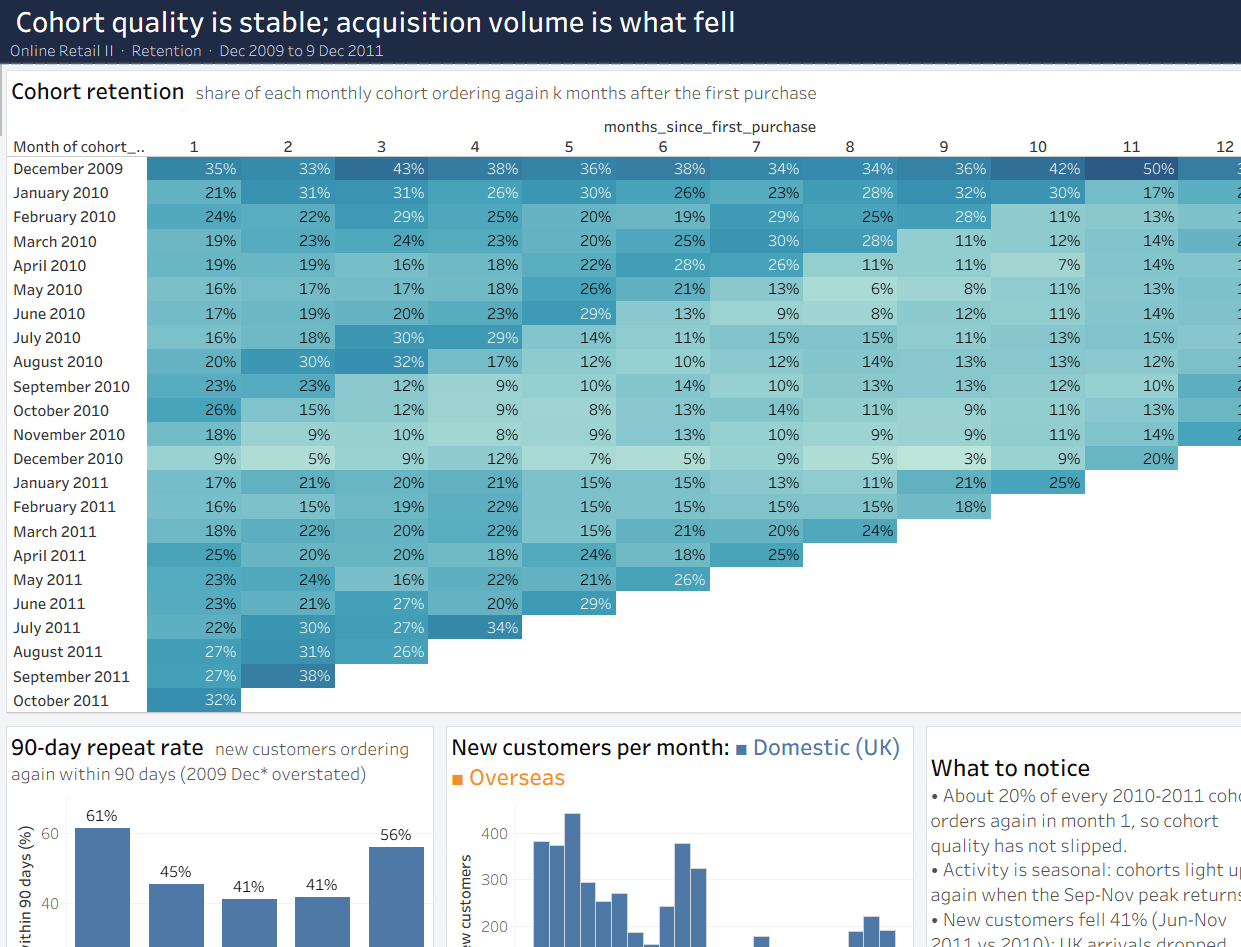
\includegraphics[width=0.95\textwidth]{tableau_retention.png}
\caption{Retention dashboard (same sheets and size as in the packaged file).}
\end{figure}
\begin{figure}[H]
\centering
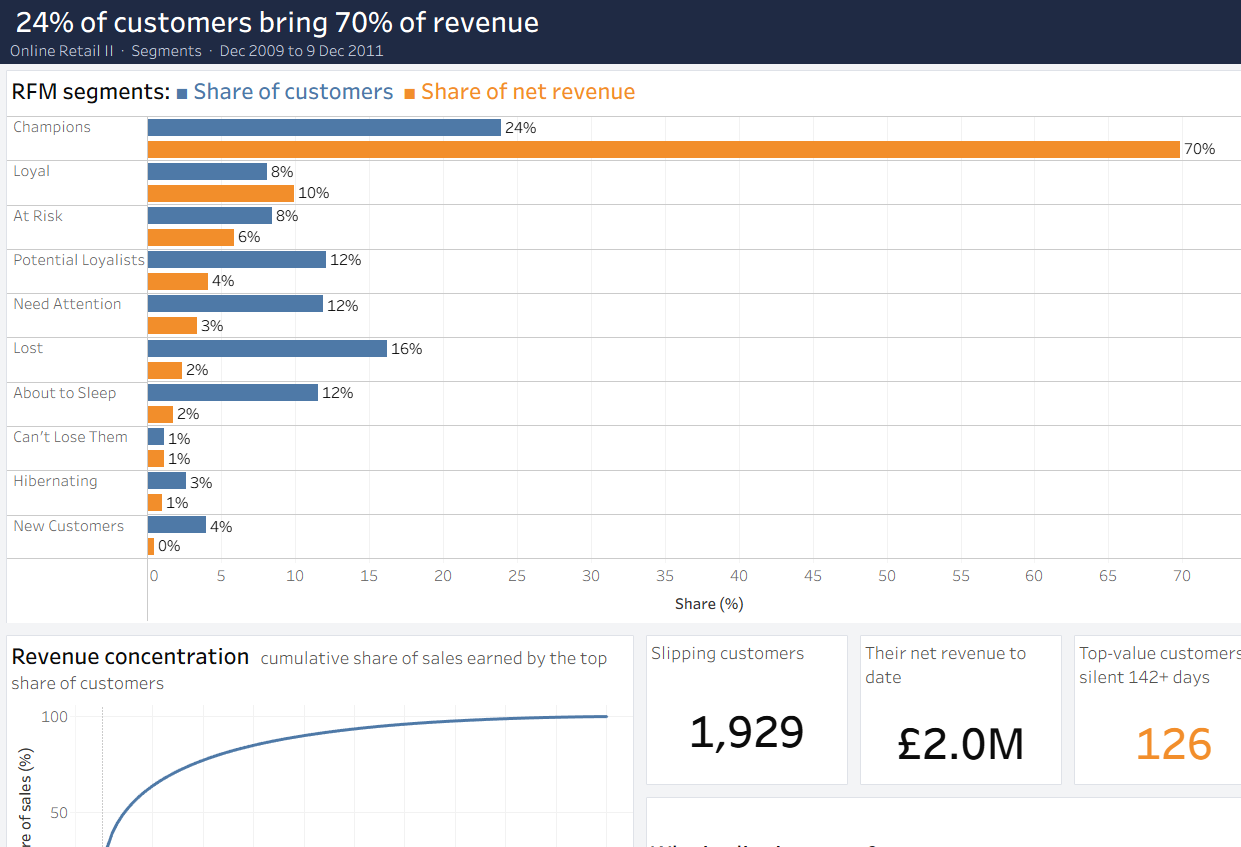
\includegraphics[width=0.95\textwidth]{tableau_segments.png}
\caption{Segments dashboard (same sheets and size as in the packaged file).}
\end{figure}
\begin{figure}[H]
\centering
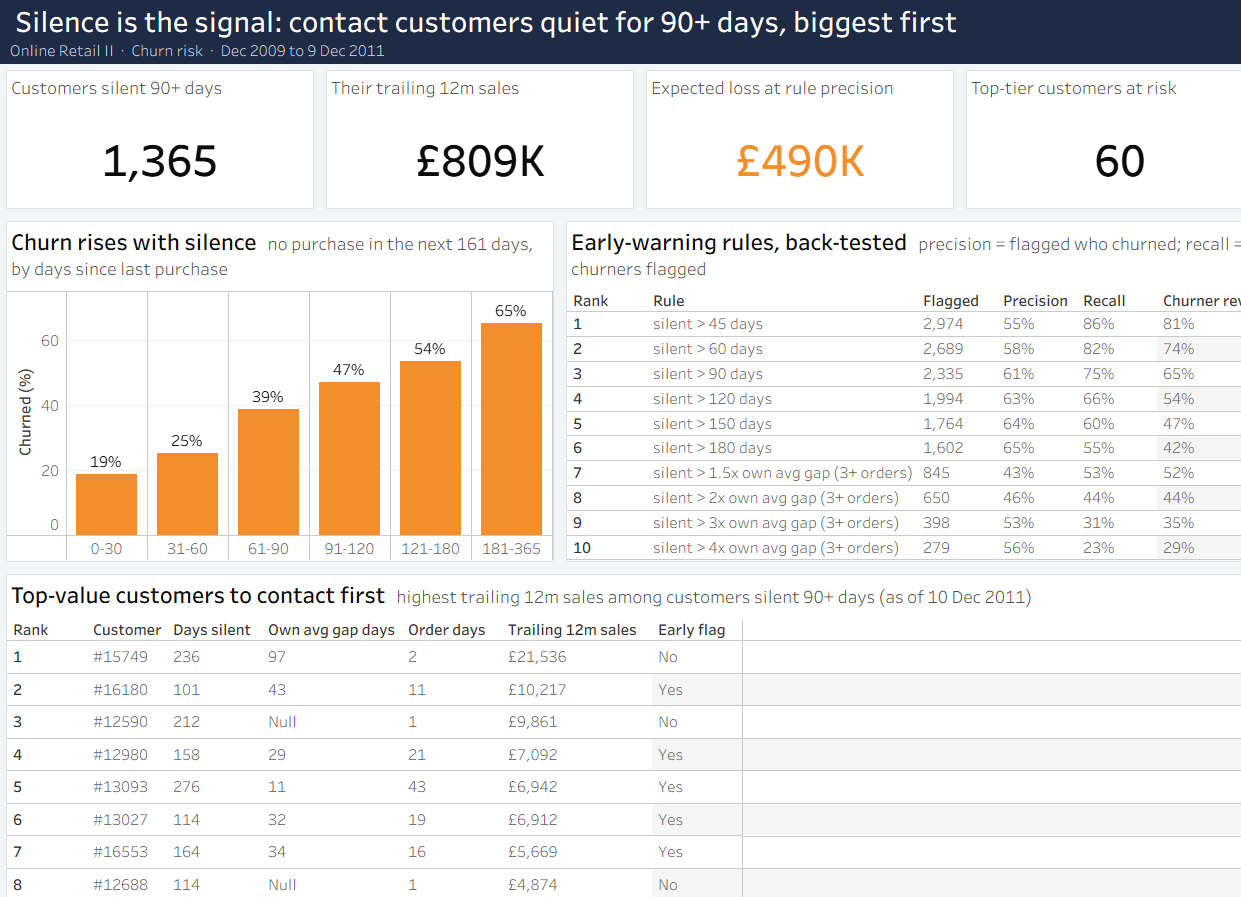
\includegraphics[width=0.95\textwidth]{tableau_churn_risk.png}
\caption{Churn risk dashboard (same sheets and size as in the packaged file).}
\end{figure}
\begin{figure}[H]
\centering
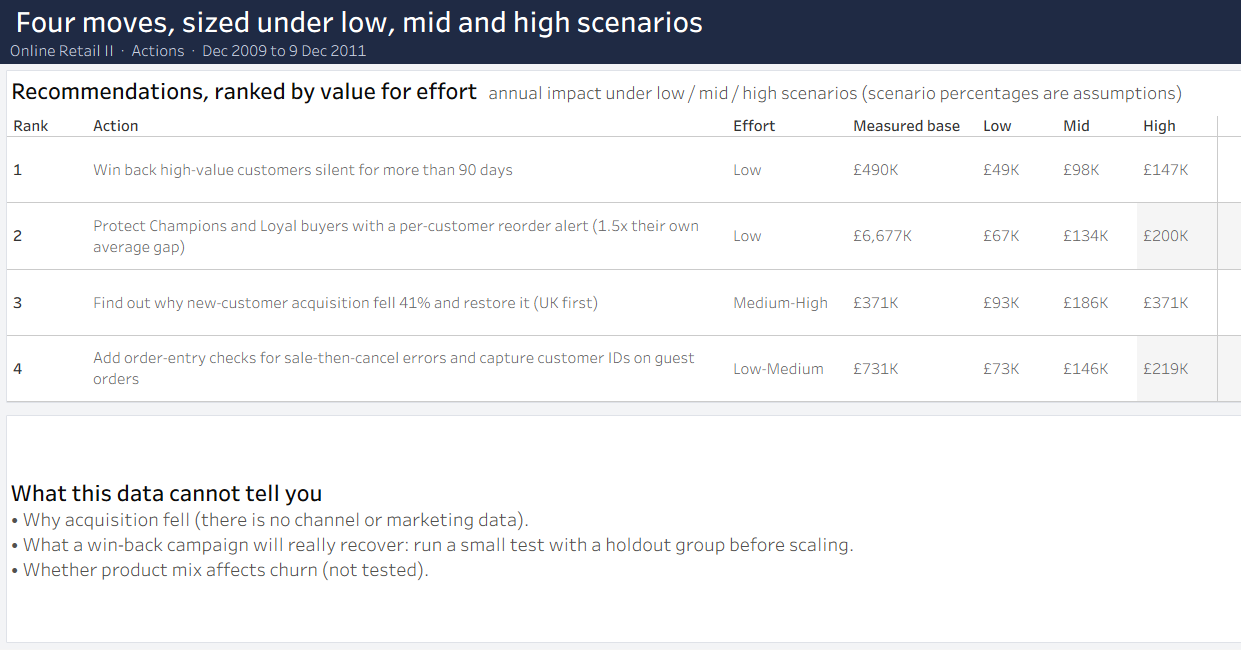
\includegraphics[width=0.95\textwidth]{tableau_actions.png}
\caption{Actions dashboard (same sheets and size as in the packaged file).}
\end{figure}

\subsection{Wording updated after notebook 11}
Five text items in the packaged workbook were revised after the robustness checks. The Retention banner now reads ``Cohort quality is stable since mid-2010'', and the Retention card notes that the 90-day repeat rate fell from 45\% to about 41\% and then held. The Overview \emph{Key insights} card says volume, not cohort quality, is the part to investigate. The \emph{What this data cannot tell you} card no longer lists product mix as untested; it says product mix adds little to churn prediction. The rule back-test subtitle notes that recall is 45--76\% at other cutoffs. Only text runs changed; the data files in the package are identical, and the previous version is kept in \file{dashboard/tableau/backup/}.

\subsection{Verification status}
Every dashboard opened in Tableau Desktop 2026.3 without errors and was checked in screenshots; the packaged file was opened from a copy in a different folder. Not directly seen: the small orange ``Overseas'' segments of the new-customers-by-region chart and the very bottom of the Overview text card.

\section{Presenting the story}
Suggested order: Overview (flat sales, acquisition down) $\rightarrow$ Retention $\rightarrow$ Segments $\rightarrow$ Churn risk (who to contact) $\rightarrow$ Actions.

%=====================================================================
\chapter{Phase 6: Act}
This project stops at a prioritised action plan. No action has been executed or measured.

\section{Proposed actions}
\begin{enumerate}[nosep]
\item \textbf{Win back silent high-value customers.} Start with the 60 top-tier customers on the live list, then everyone silent for more than 90 days.
\item \textbf{Protect the core.} Alert account managers when a Champion or Loyal customer passes 1.5$\times$ their own average gap.
\item \textbf{Investigate acquisition.} Find out what changed in 2011 and address it if the cause is fixable, starting with the UK.
\item \textbf{Tidy the leaks.} Check unusually large orders at entry and capture customer IDs on guest orders (mostly cost and data quality).
\end{enumerate}

\section{Test before scaling}
The recovery rate of a win-back campaign is unknown. Randomly split the flagged customers into a contacted group and a holdout group and compare the share who order again within 90 days. With 1,365 flagged customers the test can detect only large differences, so treat the result as indicative.

\section{Monitoring}
Track monthly: new customers (UK and overseas), 90-day repeat rate of new customers, the number and trailing sales of customers silent for 90+ days, cancellation rate and the share of sales with no customer ID.

\section{What would change the conclusions}
Channel or marketing data that explains the 2011 acquisition drop; results of a holdout test; an official product category field for the churn analysis; a longer history that removes the left-censoring of the first cohort.

%=====================================================================
\chapter{Reproducibility and maintenance}
\begin{lstlisting}
# open notebooks/run_all.ipynb and choose Run All, or from the notebooks folder:
..\.venv\Scripts\python -m nbconvert --to notebook --execute --inplace run_all.ipynb
\end{lstlisting}
The notebook \file{run_all.ipynb} runs notebooks 01--09 in order and stops at the first error (set the environment variable \texttt{RUN\_ONLY} to run a subset). Run notebook 08 before 09. Notebook 10 regenerates the tables and key numbers of this document in \file{docs/latex/generated/} from the project outputs and from the packaged workbook, so run it after the analysis, or after saving the workbook in Tableau, and then compile this document with pdfLaTeX twice. To compile online, upload \file{docs/latex/overleaf\_upload.zip}. All notebooks have been executed with saved outputs and no errors.

\appendix
\chapter{Glossary}
\begin{description}[nosep]
\item[Cohort] Customers grouped by the month of their first purchase.
\item[RFM] Recency, frequency and monetary value of a customer's purchases.
\item[Churn (here)] No purchase for 161 days after the back-test cutoff.
\item[Precision, recall, lift] Share of flagged customers who churned; share of churners flagged; precision divided by the base churn rate.
\item[Guest order] A transaction without a customer ID.
\item[Left-censoring] The data starts in December 2009, so earlier purchases are unseen.
\end{description}

\end{document}
